% Tell RStudio that weaving is to be done with the knitr package
% !Rnw weave = knitr


%\listfiles                   %% Show all files used in the book
\documentclass[10pt,krantz2]{krantz}\usepackage[]{graphicx}\usepackage[]{color}
%% maxwidth is the original width if it is less than linewidth
%% otherwise use linewidth (to make sure the graphics do not exceed the margin)
\makeatletter
\def\maxwidth{ %
  \ifdim\Gin@nat@width>\linewidth
    \linewidth
  \else
    \Gin@nat@width
  \fi
}
\makeatother

\definecolor{fgcolor}{rgb}{0.345, 0.345, 0.345}
\newcommand{\hlnum}[1]{\textcolor[rgb]{0.686,0.059,0.569}{#1}}%
\newcommand{\hlstr}[1]{\textcolor[rgb]{0.192,0.494,0.8}{#1}}%
\newcommand{\hlcom}[1]{\textcolor[rgb]{0.678,0.584,0.686}{\textit{#1}}}%
\newcommand{\hlopt}[1]{\textcolor[rgb]{0,0,0}{#1}}%
\newcommand{\hlstd}[1]{\textcolor[rgb]{0.345,0.345,0.345}{#1}}%
\newcommand{\hlkwa}[1]{\textcolor[rgb]{0.161,0.373,0.58}{\textbf{#1}}}%
\newcommand{\hlkwb}[1]{\textcolor[rgb]{0.69,0.353,0.396}{#1}}%
\newcommand{\hlkwc}[1]{\textcolor[rgb]{0.333,0.667,0.333}{#1}}%
\newcommand{\hlkwd}[1]{\textcolor[rgb]{0.737,0.353,0.396}{\textbf{#1}}}%

\usepackage{framed}
\makeatletter
\newenvironment{kframe}{%
 \def\at@end@of@kframe{}%
 \ifinner\ifhmode%
  \def\at@end@of@kframe{\end{minipage}}%
  \begin{minipage}{\columnwidth}%
 \fi\fi%
 \def\FrameCommand##1{\hskip\@totalleftmargin \hskip-\fboxsep
 \colorbox{shadecolor}{##1}\hskip-\fboxsep
     % There is no \\@totalrightmargin, so:
     \hskip-\linewidth \hskip-\@totalleftmargin \hskip\columnwidth}%
 \MakeFramed {\advance\hsize-\width
   \@totalleftmargin\z@ \linewidth\hsize
   \@setminipage}}%
 {\par\unskip\endMakeFramed%
 \at@end@of@kframe}
\makeatother

\definecolor{shadecolor}{rgb}{.97, .97, .97}
\definecolor{messagecolor}{rgb}{0, 0, 0}
\definecolor{warningcolor}{rgb}{1, 0, 1}
\definecolor{errorcolor}{rgb}{1, 0, 0}
\newenvironment{knitrout}{}{} % an empty environment to be redefined in TeX

\usepackage{alltt}
%\documentclass[11pt]{book}
%\usepackage{amsmath}
\usepackage{array}            %% nicer arrays and tables
\usepackage{times}            %% PS Times, rather than CM fonts
\usepackage[T1]{fontenc}      %% for non-alpha chars in \tt
\usepackage{sfheaders}        %% Chap/Sec headers in Helvetica
\usepackage{graphicx}         %% well, its about graphics
\usepackage{alltt}            %% for source listings
\usepackage{mdwlist}          %% Compressed list environments: itemize*, description*, etc.
\usepackage{comment}          %% Stuff commented out
\usepackage{xspace}           %% Smart spacing after tex macros
\usepackage[obeyspaces]{url}  %% URLs and pathnames
\usepackage{bm}               %% for bold math symbols (via \vec{}, \mat{})
\usepackage[tc]{titlepic}     %% Used for the cover illustration
\usepackage{showlabels}       %% Used for checking xrefs
\renewcommand{\showlabelfont}{\footnotesize\ttfamily}
\usepackage{tikz}             %% used for hyp3way.tex
% colored tables
\usepackage{xcolor,colortbl}  %% used ub Ch 01
\usepackage{multirow}
%\usepackage[traceon]{changebar}  %% When we need to show diffs
\usepackage{epigraph}         %% section quotations
\setlength{\epigraphwidth}{.8\textwidth}
%% indexing
\usepackage{index}          

\usepackage[comma]{natbib}
\renewcommand{\bibname}{References}
%\bibliographystyle{abbrvnat-apa}  % this includes URLs
\bibliographystyle{abbrvnat-apa-nourl}

%%%%%%%%%%%%%%%%%%%%%%%%%%%%%%%%%%%%%%%%%%%%%%%%%
%% Setup page style mods from krantz style
%%%%%%%%%%%%%%%%%%%%%%%%%%%%%%%%%%%%%%%%%%%%%%%%%
%

% figure/table names
\renewcommand\figurename{Figure}
\renewcommand\tablename{Table}

% override default to use chapter/section headers
\makeatletter
\def\HeadingsChapterSection{%
  \def\chaptermark##1{%
    \markboth{%
      \thechapter. ##1}{}}%
  \def\sectionmark##1{%
    \markright{%
      \thesection: ##1}}}
\HeadingsChapterSection

\def\@TableTitle{%
  \noindent
  {%
    \vbox{{\TableNumberFont Table\ \thetable}}\par\TableTitleFont\@tabletitle}}

\long\def\@makecaption#1#2{%
  \vskip\abovecaptionskip
  \sbox\@tempboxa{#1: #2}%
  \ifdim \wd\@tempboxa >\hsize
    {\FigCapFont #1:} #2\par
  \else
    \global \@minipagefalse
%    \hb@xt@\hsize{\hfil\box\@tempboxa\hfil}%
    {\FigCapFont #1:} #2\par
  \fi
  \vskip\belowcaptionskip}
\makeatother


% %% Page Headings
% %\makeatletter
% \usepackage{fancyhdr}
% \pagestyle{fancy}
% % \addtolength{\headwidth}{\marginparsep}
% % \addtolength{\headwidth}{\marginparwidth}
% % \addtolength{\headheight}{1.6pt}   %% suppress overfull \vbox chatter
% %
% %% The next two lines are only for draft printing
% %\def\infoleft{\quad [{\small\ttfamily\@filef@und}]}
% % \def\infoleft{[\number\month-\number\day-\number\year]\quad}
% % \def\inforight{[\number\month-\number\day-\number\year]\quad}
% %
% \renewcommand{\chaptermark}[1]{%
%  \markboth{\thechapter\ #1}{}}
% \renewcommand{\sectionmark}[1]{%
%  \markright{\thesection\ #1}}
% % \lhead[\fancyplain{}{\bfseries\sffamily\thepage}]%
% %       {\fancyplain{}{{\bfseries\sffamily\rightmark}\infoleft}}
% % \rhead[\fancyplain{}{\inforight{\bfseries\sffamily\leftmark}}]%
% %       {\fancyplain{}{\bfseries\sffamily\thepage}}
% % \cfoot{}
% %\makeatother

%%%%%%%%%%%%%%%%%%%%%%%%%%%%%%%%%%%%%%%%%%%%%%%%
%% Indexing -- only main index for now
%%%%%%%%%%%%%%%%%%%%%%%%%%%%%%%%%%%%%%%%%%%%%%%%

%\makeglossary
\usepackage{index}
\makeindex
\newindex{xmp}{ide}{ine}{Example Index}

% %% Page Headings
% \makeatletter
% \usepackage{fancyhdr}
% \pagestyle{fancy}
% \addtolength{\headwidth}{\marginparsep}
% \addtolength{\headwidth}{\marginparwidth}
% \addtolength{\headheight}{1.6pt}   %% suppress overfull \vbox chatter
% %
% %% The next two lines are only for draft printing
% \def\infoleft{\quad [{\small\ttfamily\@filef@und}]}
% \def\inforight{[\number\month-\number\day-\number\year]\quad}
% %
% \renewcommand{\chaptermark}[1]{%
%  \markboth{\thechapter\ #1}{}}
% \renewcommand{\sectionmark}[1]{%
%  \markright{\thesection\ #1}}
% \lhead[\fancyplain{}{\bfseries\sffamily\thepage}]%
%       {\fancyplain{}{{\bfseries\sffamily\rightmark}\infoleft}}
% \rhead[\fancyplain{}{\inforight{\bfseries\sffamily\leftmark}}]%
%       {\fancyplain{}{\bfseries\sffamily\thepage}}
% \cfoot{}
% \makeatother

%%%%%%%%%%%%%%%%%%%%%%%%%%%%%%%%%%%%%%%%%%%%%%%%
% Only for chapter.Rnw
\usepackage{xr}
\externaldocument{book}
%%%%%%%%%%%%%%%%%%%%%%%%%%%%%%%%%%%%%%%%%%%%%%%%


% %  Page dimensions
% \addtolength{\hoffset}{-1.1cm}
% \addtolength{\textwidth}{2.2cm}
% \addtolength{\voffset}{-2cm}
% \addtolength{\textheight}{4cm}
% \setlength{\parskip}{3pt plus 1pt}
% \addtolength\marginparwidth {-.5cm}
% 
% % Float parameters
% \renewcommand\textfraction{.15}
% \renewcommand\topfraction{.8}
% % the rest are the defaults
% \setcounter{topnumber}{2}
% \setcounter{bottomnumber}{1}
% \renewcommand\bottomfraction{.3}
% \setcounter{totalnumber}{3}
% \renewcommand\floatpagefraction{.5}

% General LaTeX commands for VCDR

%  Math commands
\newcommand{\bvec}[1]{\ensuremath{\mathbf{#1}}}
\renewcommand{\vec}[1]{\ensuremath{\bm{#1}}}
%\newcommand{\mat}[1]{\ensuremath{\mathbf{#1}}}
\newcommand{\mat}[1]{\ensuremath{\bm{#1}}}               % matrix (bold)
\newcommand{\trans}{\ensuremath{^\mathsf{T}}}            % transpose
\newcommand*{\degree}[1]{\ensuremath{{#1}^{\circ}}}
\newcommand{\diag}[1]{\ensuremath{\mathrm{diag}\, #1}}
\def\binom#1#2{{#1 \choose #2}}%
\newcommand*{\comma}{\:\: ,}%                      punct after displaymath
\newcommand*{\period}{\:\: .}
\newcommand*{\given}{\ensuremath{\, | \,}}
\newcommand*{\implies}{\ensuremath{\Longrightarrow}}

\newcommand*{\rank}[1]{\ensuremath{\mathrm{rank} (\mat{#1})}}
\newcommand*{\dev}[1]{(#1 - \bar{#1})}
\newcommand*{\inv}[1]{\ensuremath{\mat{#1}^{-1}}}
\newcommand*{\half}[1]{\ensuremath{\mat{#1}^{1/2}}}
\newcommand*{\nvec}[2]{\ensuremath{{#1}_{1}, {#1}_{2},\ldots,{#1}_{#2}}}
\newcommand*{\E}{\mathcal{E}}
\newcommand*{\V}{\mathcal{V}}
\newcommand{\iid}{\stackrel{iid}{\sim}}

\newcommand{\blacksquare}{\rule{1.4ex}{1.4ex}}

% Coefficient with error underneath
\newcommand{\cwe}[2]{% 
  \mathord{\mathop{#1}\limits_{(#2)}}%
}
\newcommand{\sizedmat}[2]{%
  \mathord{\mathop{\mat{#1}}\limits_{(#2)}}%
}

%%%%%%%%%%%%%%%%%%%%%%%%%%%%%%%%%%%%%%%%%%%%%%%%%%%%%%
% mathematical functions
%%%%%%%%%%%%%%%%%%%%%%%%%%%%%%%%%%%%%%%%%%%%%%%%%%%%%%

\makeatletter
\def\logit{\mathop{\operator@font logit}}
\def\Bin{\mathop{\operator@font Bin}}
\def\Pois{\mathop{\operator@font Pois}}
\def\NBin{\mathop{\operator@font NBin}}
\def\Geom{\mathop{\operator@font Geom}}
\def\sign{\mathop{\operator@font sign}}
\def\Vec{\mathop{\operator@font vec}}

%\newcommand{\min}{\operatornamewithlimits{min}}
%\newcommand{\max}{\operatornamewithlimits{max}}
%\newcommand{\argmin}{\operatornamewithlimits{arg\,min}}
%\newcommand{\argmax}{\operatornamewithlimits{arg\,max}}
% the *ed form allows limits above/below, the non*ed form prints these beside the operator
%\DeclareMathOperator*{\argmin}{arg\,min}

%\newcommand{\Xvec}{X_1,X_2, \ldots, X_n }
% should add an argument for n
\newcommand{\sumi}[2]{\sum_{#1=1}^#2}

\def\ignorespacesafterend{\global\@ignoretrue}
\newenvironment{equation*}
	{\begin{displaymath}}%
%	{\end{displaymath}}%
	{\end{displaymath}\ignorespacesafterend}%
%
% Donald Arseneau recommends:
%\newenvironment{equation*}{\displaymath}{\enddisplaymath}%

%%%%%%%%%%%%%%%%%%%%%%%%%%%%%%%%%%%%%%%%%%%%%%%%%%%%%%
%% common abbreviations
%%%%%%%%%%%%%%%%%%%%%%%%%%%%%%%%%%%%%%%%%%%%%%%%%%%%%%

\newcommand*{\hires}{high-resolution}
\newcommand*{\etal}{\emph{et al.}}
\newcommand*{\loglin}{loglinear\xspace}
\newcommand*{\Loglin}{Loglinear\xspace}
\newcommand*{\ctab}{contingency table\xspace}
\newcommand*{\ctabs}{contingency tables\xspace}
\newcommand*{\mway}{multiway\xspace}
\newcommand*{\LR}{likelihood-ratio\xspace}
\newcommand*{\CA}{Correspondence analysis\xspace}
\newcommand*{\ca}{correspondence analysis\xspace}
\newcommand*{\nway}{\emph{n}-way\xspace}
\newcommand*{\GSQ}{\ensuremath{G^2}\xspace}
\newcommand*{\chisq}{\ensuremath{\chi^2}\xspace}
\newcommand*{\scat}{scatterplot\xspace}
\newcommand*{\scats}{scatterplots\xspace}
\newcommand*{\scatmat}{\scat{} matrix\xspace}
\newcommand*{\df}{degrees of freedom\xspace}
\newcommand*{\Dset}{data set\xspace}
\newcommand*{\Dsets}{data set\xspace}

%% notation for loglinear models [AB][C] -- now use \mathrm{}
\newcommand*{\llmterm}[1]{\ensuremath{[}#1\ensuremath{]}}
%\newcommand*{\llmterm}[1]{\ensuremath{[}\ensuremath{\mathrm{#1}\ensuremath{]}}
%\newcommand*{\llmterm}[1]{\ensuremath{[\mathrm{#1}]}
\newcommand*{\llmtwo}[2]{\llmterm{#1} \llmterm{#2}}
\newcommand*{\llmthree}[3]{\llmterm{#1} \llmterm{#2} \llmterm{#3}}
\newcommand*{\llmfour}[4]{\llmterm{#1} \llmterm{#2} \llmterm{#3} \llmterm{#4}}

%% \LLM{A,B,C} --> [A] [B] [C] for loglin models
\DeclareRobustCommand*{\LLM}[1]{%
%\def\LLM#1{%
	\@for\@term:=#1\do{%
	\llmterm{\@term}%
	}
}
\makeatother

% deprecated, but maybe used somewhere
\newcommand*{\boldital}[1]{\textit{\textbf{#1}}}

%%%%%%%%%%%%%%%%%%%%%%%%%%%%%%%%%%%%%%%%%%%%%%%%%%%%%%%%%%%%%%%%%%
% precept -- something to stand out in the text
%   could use a box or something else
%%%%%%%%%%%%%%%%%%%%%%%%%%%%%%%%%%%%%%%%%%%%%%%%%%%%%%%%%%%%%%%%%%

\newcommand{\precept}[1]{%
\begin{quote}
\centering
\textbf{#1}
\end{quote}
}


%%%%%%%%%%%%%%%%%%%%%%%%%%%%%%%%%%%%%%%%%%%%%%%%%%%%%%%%%%%%%%%%%%
% \glossterm -- used for terms that should be highlighted in the
% text and index, and which might go into a glossary (but only 
% if glosstex is run)
% The original definition did not allow for such terms at the beginning
% of a sentence.
%\newcommand{\glossterm}[1]{\textit{\textbf{#1}}\glosstex{#1}}

% Simple variant, just for formatting; can also use \marginpar{}
% and glossterm
\newcommand{\term}[1]{\textit{\textbf{#1}}\index{#1}}

%\glossterm[print-form]{gloss-form}
\makeatletter
\def\glossterm{\@dblarg\@glossterm}
\def\@glossterm[#1]#2{\textit{\textbf{#1}}\glosstex{#2}\index{#2|textbf}}
\makeatother

% Author's notes -- to disappear in production
\newcommand{\aunote}[1]{\marginpar{\footnotesize\textbf{Au:} #1}}

% Dummy command for changes
%\newenvironment{changebar}{}{}%
%\newcommand{\changebar}[1]{#1}

%%%%%%%%%%%%%%%%%%%%%%%%%%%%%%%%%%%%%%%%%%%%%%%%%%%%%%%%%%%%%%%%%%%%%%
% Commands to simplify cross-references
%%%%%%%%%%%%%%%%%%%%%%%%%%%%%%%%%%%%%%%%%%%%%%%%%%%%%%%%%%%%%%%%%%%%%%

\newcommand*{\eqref}[1]{Eqn.~(\ref{#1})}
\newcommand*{\exref}[1]{Example~\ref{#1}}
\newcommand*{\chref}[1]{Chapter~\ref{#1}}
\newcommand*{\secref}[1]{Section~\ref{#1}}
\newcommand*{\figref}[1]{Figure~\ref{#1}}
\newcommand*{\tabref}[1]{Table~\ref{#1}}
\newcommand*{\outref}[1]{Output~\ref{#1}}
\newcommand*{\datref}[1]{Appendix~\ref{#1}}
%\newcommand*{\macref}[1]{Appendix~\ref{#1}}
\newcommand*{\appref}[1]{Appendix~\ref{#1}}

% Reference a range of refs
\newcommand*{\chrange}[2]{Chapters~\ref{#1}--\ref{#2}}
\newcommand*{\figrange}[2]{Figures~\ref{#1}--\ref{#2}}
\newcommand*{\tabrange}[2]{Tables~\ref{#1}--\ref{#2}}
%
% Reference a list of figs, examples, etc., not necessarily sequential
\newcommand{\figrefs}[1]{\dorefs{#1}{Figures}}
\newcommand{\tabrefs}[1]{\dorefs{#1}{Tables}}
\newcommand{\exrefs}[1]{\dorefs{#1}{Examples}}
\makeatletter
\newcommand{\dorefs}[2]{%
  \let\@dummy\@empty
  #2~%
  \@for\@term:=#1\do{%
    \@dummy
    \edef\@dummy{\ref{\@term}, }}%
  \expandafter\format@last\@dummy}
\def\format@last#1, {and #1}
\makeatother


%%%%%%%%%%%%%%%%%%%%%%%%%%%%%%%%%%%%%%%%%%%%%%%%%%%%%%%%%%%%%%%%%%%%%%%%%%%
% multiline headers in tables 
% use as: Variable & DF & \multilineC{Parameter \\ Estimate} & ...
%%%%%%%%%%%%%%%%%%%%%%%%%%%%%%%%%%%%%%%%%%%%%%%%%%%%%%%%%%%%%%%%%%%%%%%%%%%

\newcommand{\multilineR}[1]{\begin{tabular}[b]{@{}r@{}}#1\end{tabular}} 
\newcommand{\multilineL}[1]{\begin{tabular}[b]{@{}l@{}}#1\end{tabular}} 
\newcommand{\multilineC}[1]{\begin{tabular}[b]{@{}c@{}}#1\end{tabular}} 

%% table stuff, another way
% to make it easier to use & \brk{this\\or\\that} & in \tabular

\newcommand{\brk}[2][l]{%
   \begin{tabular}{@{}#1@{}}#2%
   \end{tabular}%
}

%%%%%%%%%%%%%%%%%%%%%%%%%%%%%%%%%%%%%%%%%%%%%%%%%%%%%%%%%%%%%%%%%%%%%%%%%%%%
% colored tables
%%%%%%%%%%%%%%%%%%%%%%%%%%%%%%%%%%%%%%%%%%%%%%%%%%%%%%%%%%%%%%%%%%%%%%%%%%%%
% requires:
%\usepackage{xcolor,colortbl}  %% used ub Ch 01

%\newcommand{\tableheader}{\rowcolor[gray]{.85}}
\newcommand{\tableheader}{\rowcolor[HTML]{FFFFC7}} % light yellow background

\newcommand{\cell}[2]{\multicolumn{1}%
   {>{\columncolor{#1}}r}{#2}}

\newcommand{\C}{Chapter\xspace}

\newcommand{\chapterprelude}[1]{%
\textsf{#1}
\newline
\rule{\textwidth}{0.4pt}
}


%\renewcommand{\S}{Section }

%%%%%%%%%%%%%%%%%%%%%%%%%%%%%%%%%%%%%%%%%%%%%%%%%%%%%%%%%%%%%%%
% R terminology

% writing about R stuff; these can be modified to add indexing, etc.
\newcommand{\var}[1]{\texttt{#1}}

% Data sets -- print and index
%\newcommand{\data}[1]{\texttt{#1}}
\newcommand*{\data}[1]{\textit{\texttt{#1}}\ixd{#1}}

\newcommand{\class}[1]{\textsf{"#1"}}

% may need a more robust version of \code to handle special chars
% this doesn't quite handle it.
% Added \sloppy to avoid \hbox too wide problems
\makeatletter
\newcommand\code{\bgroup\@makeother\_\@makeother\~\@makeother\$\@codex}
\def\@codex#1{{\sloppy\normalfont\ttfamily\hyphenchar\font=-1 #1}\egroup}
\makeatother
%\newcommand{\code}[1]{\texttt{#1}}

% R functions: use \code{} and also \index{}
\newcommand{\func}[1]{\code{#1()}\ixfunc{#1}}

\let\proglang=\textsf
\newcommand{\R}{\proglang{R}\xspace}

% should redefine \pkg to also cite the package, but this requires
% an extra, optional argument, unless it is assured that the package
% name is the bibtex key; also: add indexing
%\newcommand{\pkg}[1]{{\normalfont\fontseries{b}\selectfont #1}}
%\newcommand{\pkg}[1]{\textsf{#1}\ixp{#1}}

% reference and \cite a package, but only on first use
\def\pkg#1{\textsf{#1}\ixp{#1}~\citex{#1}\xspace}
\def\citex#1{\expandafter\ifx\csname cit:#1\endcsname\relax
      \expandafter\gdef\csname cit:#1\endcsname{}%
      \citep{#1}%
   \else
      \nocite{#1}%
   \fi
}

\newcommand{\Rpackage}[1]{\pkg{#1} package}

% R base packages all have the same reference -- shouldn't be cited
\newcommand{\basepkg}[1]{\textsf{#1}\ixp{#1}}



\newcommand{\help}[1]{\code{help(#1)}}     % reference R help

\newcommand*{\VCDR}{\emph{VCDR} }
\newcommand*{\argument}[1]{\texttt{#1} argument}
%\newcommand*{\sasprog}[1]{\texttt{#1} program\ixp{#1}}
%\newcommand*{\default}[1]{\texttt{[}Default: \url{#1}\texttt{]}}

%%%%%%%%%%%%%%%%%%%%%%%%%%%%%%%%%%%%%%%%%%%%%%%%%%%%%%%%%%%%%%%%%%%%%%%
% Index generation
% Indexentry for a word/phrase (Word inserted into the text)
%%%%%%%%%%%%%%%%%%%%%%%%%%%%%%%%%%%%%%%%%%%%%%%%%%%%%%%%%%%%%%%%%%%%%%%
\newcommand{\IX}[1]{\index{#1}#1}
\newcommand{\ix}[1]{\index{#1}}
\newcommand{\ixmain}[1]{\index{#1|textbf}}

%\newcommand{\ixm}[1]{%
%   \index{#1@\texttt{#1} macro}%
%   \index{macros!#1@\texttt{#1}}%
%	}

% R functions
\newcommand{\ixfunc}[1]{%
  \index{#1@\texttt{#1()}}%
%  \index{functions!#1@\texttt{#1}}%
 }

% R packages:  indexed under both package name and packages!
\newcommand{\ixp}[1]{%
   \index{#1@\textsf{#1} package}%
   \index{package!#1@\textsf{#1}}%
	}


% data sets: 
\newcommand{\ixd}[1]{%
        \index{data sets!#1}}

% Examples Index
\newcommand{\ixe}[1]{\index[xmp]{#1}}
\newcommand{\ixeon}[1]{\ixe{#1|(}}      % when not automatically done by Example
\newcommand{\ixeoff}[1]{\ixe{#1|)}}

\newcommand{\ixon}[1]{\index{#1|(}}
\newcommand{\ixoff}[1]{\index{#1|)}}


%\newcommand*\seealso[2]{\emph{\alsoname} #1}
% and then:
%\index{foo|seealso{bar}}
% If \alsoname isn't defined, you would have to add:
%\newcommand{\alsoname}{see also}

% This puts the argument in italics in the text, in boldface in the
% index, and if you give an optional argument, that goes in the index,
% so you can write:

%\define{gnat}
%\define[animals|gnats]{gnat}

\makeatletter
\newcommand{\define}{\@ifnextchar[\@dfna\@dfnb}
\def\@dfna[#1]#2{\textit{#2}\index{#1|textbf}}
\def\@dfnb#1{\@dfna[#1]{#1}}
\makeatother

%%%%%%%%%%%%%%%%%%%%%%%%%%%%%%%%%%%%%%%%%%%%%%%%%%%%%%%%%%%%%%%%%%%%%%%%%%%
% Some convenience macros for figures --- not used here
% because knitr seems to do things reasonably well without them.

% Define the current fig directory
\newcommand{\figdir}{ch\thechapter/fig/}
% Redefine the current fig directory
\newcommand{\newfigdir}[1]{\renewcommand{\figdir}{#1/fig/}}

% Command to collect graphics file info - ignored for now, but used
% whereever I abbreviate the graphics file 
% from {chX/fig/figure.eps} to {figure}
\newcommand{\graphicsfile}[2]{\relax}

%% \SASfig{file}{include_opts}{label}{caption}
%  This command is no longer used -- all figures use \includegraphics directly

%\newcommand{\SASfig}[4]{%
%  \centering%
%  \includegraphics[#2]{#1}\graphicsfile{\figdir#1}{}%
%  \caption{#4}\label{fig:#3}%
%  }

%% \fig{file}{include_opts}{shortcaption}[extended caption]
%  label is fig:file
\makeatletter
  \newcommand{\fig}[3]{\@ifnextchar[%]
    {\@extr@fig{#1}{#2}{#3}}%
    {\@norm@fig{#1}{#2}{#3}}%
  }
  \def\@extr@fig#1#2#3[#4]{%
    \begin{figure}[htb]%
    \centering%
    \includegraphics[#2]{\figdir#1}%
    \caption[#3]{#3. #4}\label{fig:#1}%
    \end{figure}%
    }
  \newcommand{\@norm@fig}[3]{%
    \begin{figure}[htb]%
    \centering%
    \includegraphics[#2]{\figdir#1}%
    \caption{#3}\label{fig:#1}%
    \end{figure}%
    }


%%%%%%%%%%%%%%%%%%%%%%%%%%%%%%%%%%%%%%%%%%%%%%%%%%%%%%%%%%%%%%%%%%%%%%%%%%
% Specialized kinds of lists
%%%%%%%%%%%%%%%%%%%%%%%%%%%%%%%%%%%%%%%%%%%%%%%%%%%%%%%%%%%%%%%%%%%%%%%%%%


% APA Seriations: ONE level of seriation only.
%  \begin{seriate} \item ... \end{seriate}
%           within a paragraph or sentence

\newcounter{APAenum}
\def\seriate{\@bsphack\begingroup%
   \setcounter{APAenum}{0}%
   \def\item{\addtocounter{APAenum}{1}(\alph{APAenum})\space}%
   \ignorespaces}
\def\endseriate{\endgroup\@esphack}

\makeatother

% definition lists for programs or arguments, with suitable indenting

\newenvironment{proglist}%
 {\begin{list}{}{%
    \settowidth{\labelwidth}{\texttt{PROGRAMSxx}}
         \setlength{\leftmargin}{\labelwidth}
         \addtolength{\leftmargin}{\labelsep}
         \setlength{\parsep}{0.2ex plus0.2ex minus0.2ex}
         \setlength{\itemsep}{0pt}
         \renewcommand{\makelabel}[1]{\texttt{##1\hfill}}}}
 {\end{list}}


%%%%%%%%%%%%%%%%%%%%%%%%%%%%%%%%%%%%%%%%%%%%%%%%%%%%%%%%%%%%%%%%%%%%%%%
% Numbered examples that can be referenced
%%%%%%%%%%%%%%%%%%%%%%%%%%%%%%%%%%%%%%%%%%%%%%%%%%%%%%%%%%%%%%%%%%%%%%%
%
% \newcounter{example}[chapter]
% \renewcommand{\theexample}{\thechapter.\arabic{example}}
% \newenvironment{Example}[2][\theexample]{%
%   \refstepcounter{example}%
%   \label{ex:#1}%
%   \def\theexamplename{#2}%
%   \begin{trivlist}%
%   \item[%
%   % \hskip-\labelsep % idiosyncrasy that needs learning
%     \textbf{\textsc{Example \theexample}:}] %
% 	\textbf{#2}\par
%   \ixe{#2|(}%
%   }{%
% 	\expandafter\ixe\expandafter{\theexamplename|)}%   magic from Bernd
%   \hfill$\triangle$
% %  The triangle used to mark the end of examples can be replaced by any
% %  other character, ... e.g.,
% %  \hfill\blacksquare
% %	\ding{110}% filled black square (using pifont package)
%   \end{trivlist}%
% }
%%%%%%%%%%%%%%%%%%%%%%%%%%%%%%%%%%%%%%%%%%%%%%%%%%%%%%%%%%%%%%%%%%%%%%%
% Numbered examples that can be referenced and produce index entries
%%%%%%%%%%%%%%%%%%%%%%%%%%%%%%%%%%%%%%%%%%%%%%%%%%%%%%%%%%%%%%%%%%%%%%%
%
\usepackage{xparse}

  \newcounter{example}[chapter]
	\renewcommand{\theexample}{\thechapter.\arabic{example}}
	\NewDocumentEnvironment{Example}{+O{\theexample}+m+o}{%
	  \refstepcounter{example}%
	  \label{ex:#1}%
	  \def\theexamplename{#2}%
	  \begin{trivlist}%
	  \item[%
	  % \hskip-\labelsep % idiosyncrasy that needs learning
	    \textbf{\textsc{Example \theexample}:}] %
	    \IfValueTF{#3}{%
	    \textbf{#2 -- #3}\par
	      \index[xmp]{#2!#3|(}
	    }{%
	    \textbf{#2}\par
	      \index[xmp]{#2|(}
	    }}{%
	    \IfValueTF{#3}{%
	      \index[xmp]{#2!#3|)}
	    }{%
	      \index[xmp]{#2|)}
	    }
	    \hfill$\triangle$
	  \end{trivlist}%
	}

%%%%%%%%%%%%%%%%%%%%%%%%%%%%%%%%%%%%%%%%%%%%%%%%%%%%%%%%%%%%%%%%%%
% Define new list type for exercises
% from: http://tex.stackexchange.com/questions/196199/exercise-list-using-enumitem-how-control-indentation-and-labeling-of-sublists
% by: Daniel Wunderlich
%%%%%%%%%%%%%%%%%%%%%%%%%%%%%%%%%%%%%%%%%%%%%%%%%%%%%%%%%%%%%%%%%%
%
\usepackage{enumitem}      % this should be loaded in book.Rnw
%
\newlist{Exercises}{enumerate}{2}
% set list style parameters
\setlist[Exercises]{%
  label=\textbf{Exercise \thechapter.\arabic*}~,  % Label: Exercise Chapter.exercise
  ref=\thechapter.\arabic*, % References: Chapter.exercise (important!)
  align=left,               % Left align labels
  labelindent=0pt,          % No space betw. margin of list and label
  leftmargin=0pt,           % No space betw. margin of list and following lines
  itemindent=!,             % Indention of item computed automatically
  itemsep=3pt,
}

\newcommand{\exercise}{%
  \item\label{lab:\arabic{chapter}.\arabic{Exercisesi}}%      % Append label to item
  \setlist[enumerate, 1]{label=(\alph*),itemsep=0pt}          % Label for subexercises, but only within an exercise
}

% references to exercises
\newcommand{\labref}[1]{Exercise~\ref{#1}}

%%%%%%%%%%%%%%%%%%%%%%%%%%%%%%%%%%%%%%%%%%%%%%%%%%%%%%%%%%%%%%%%%%%%
%  Author notes, etc

\newcommand{\TODO}[1]{\noindent{\color{red}\textbf{TODO}: #1}}
\newcommand{\DONE}[1]{\noindent{\color{blue}\textbf{Done}: #1}}
% convert these to ignore the supplied text when no longer needed
%\newcommand{\TODO}[1]{\relax}
%\newcommand{\DONE}[1]{\relax}



%% Latex notes, p 73
\newlength{\boxedparwidth}
\setlength{\boxedparwidth}{.92\textwidth}
\newenvironment{boxedtext}%
        {\begin{center}%
         \begin{tabular}{|@{\hspace{.15in}}c@{\hspace{.15in}}|}
         \hline \\ begin{minipage}[t]{\boxedparwidth}
         }
         {\end{minipage} \\ \\ \hline \end{tabular} \end{center}}




%%%%%%%%%%%%%%%%%%%%%%%%%%%%%%%%%%%%%%%%%%%%%%%%%%%%%%%%%%%%%%%%%%%%%%
% Symbols for hard or difficult sections and problems

% -- tried using \dbend, a la TeXbook, but it doesn't look right
% \usepackage{manfnt}
% \newcommand{\hard}{\marginpar{\dbend}}
% \newcommand{\veryhard}{\marginpar{\dbend \dbend}}

\newcommand{\hard}{$^\star$\xspace}
\newcommand{\veryhard}{$^{\star\star}$\xspace}

% need these for exercises
% see http://tex.stackexchange.com/questions/223505/marking-hard-exercises-in-a-book-with-enumitem
\newcommand{\exhard}{\hspace*{-\labelsep}\hard}
\newcommand{\exveryhard}{\hspace*{-\labelsep}\veryhard}


\endinput

\renewenvironment{knitrout}{\small\renewcommand{\baselinestretch}{.85}}{} % an empty environment to be redefined in TeX

%% Shut up some overfull hboxes
\hfuzz=12pt

%%%%  end{preamble}   %%%%%


% % Ch 1
% \setcounter{chapter}{0} % one less than chapter number
% \setcounter{page}{0}    % one less than book page number
% 
% % Ch 2
% \setcounter{chapter}{1} % one less than chapter number
% \setcounter{page}{18}   % one less than book page number
% 
% % Ch 3
% \setcounter{chapter}{2} % one less than chapter number
% \setcounter{page}{50}   % one less than  book page number
% 

%%%%%%%%%%%%%%%%%%%%%%%%%%%%%%%%%%%%%%%%%%%%%%%%%%%%%%%%%%%%%%%%%%%%%%%%%
% Set chapter number in this chunk; edit the page numbers as they change

\setcounter{chapter}{0}\setcounter{page}{0}

\IfFileExists{upquote.sty}{\usepackage{upquote}}{}
\begin{document}




\chapter{Introduction}\label{ch:intro}
%\begin{center}
 \rule[-4pt]{0.5pt}{4pt}\hrulefill\rule[-4pt]{0.5pt}{4pt}\\
 \begin{minipage}[c]{.33\linewidth}
  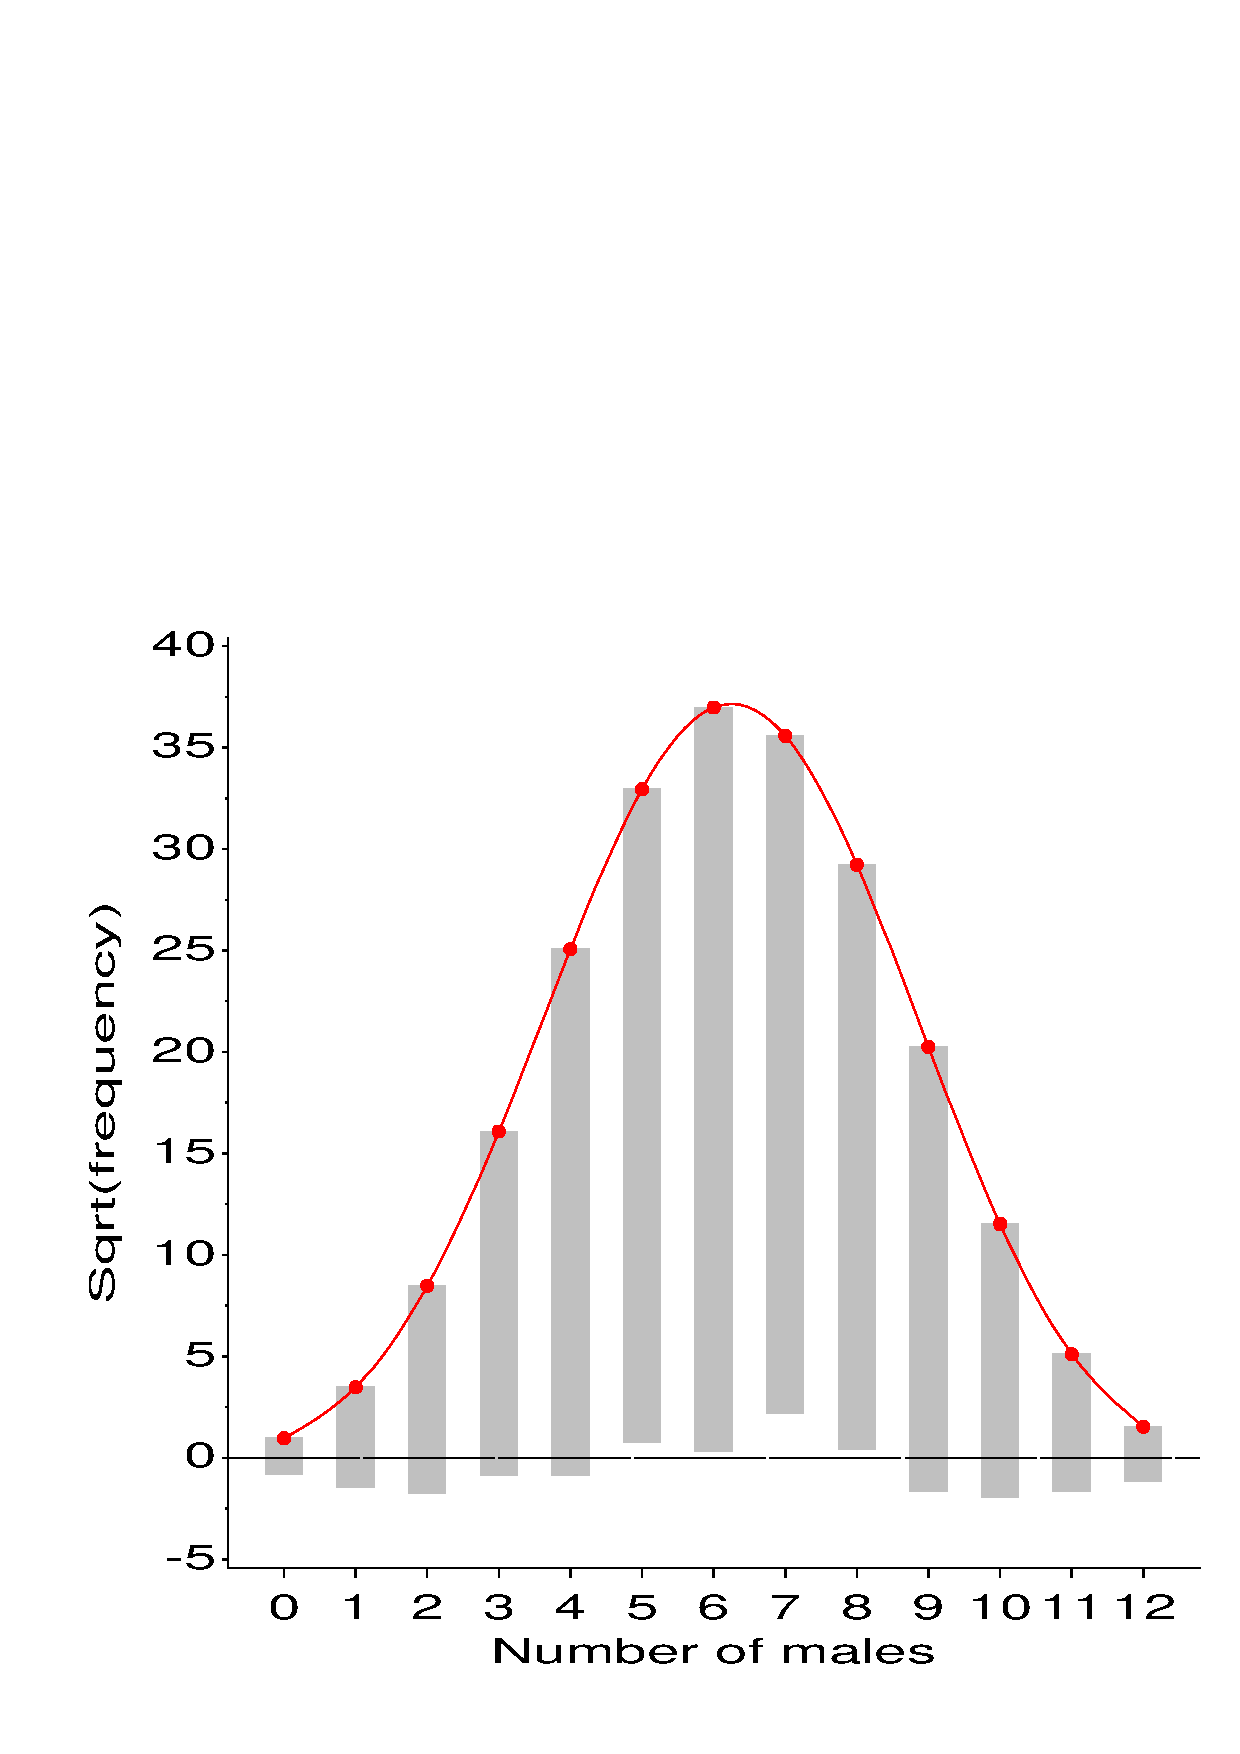
\includegraphics[width=1\linewidth]{saxony}\graphicsfile{ch2/fig/saxony.eps}{}
 \end{minipage}%
 \hfill
 \begin{minipage}[c]{.33\linewidth}
  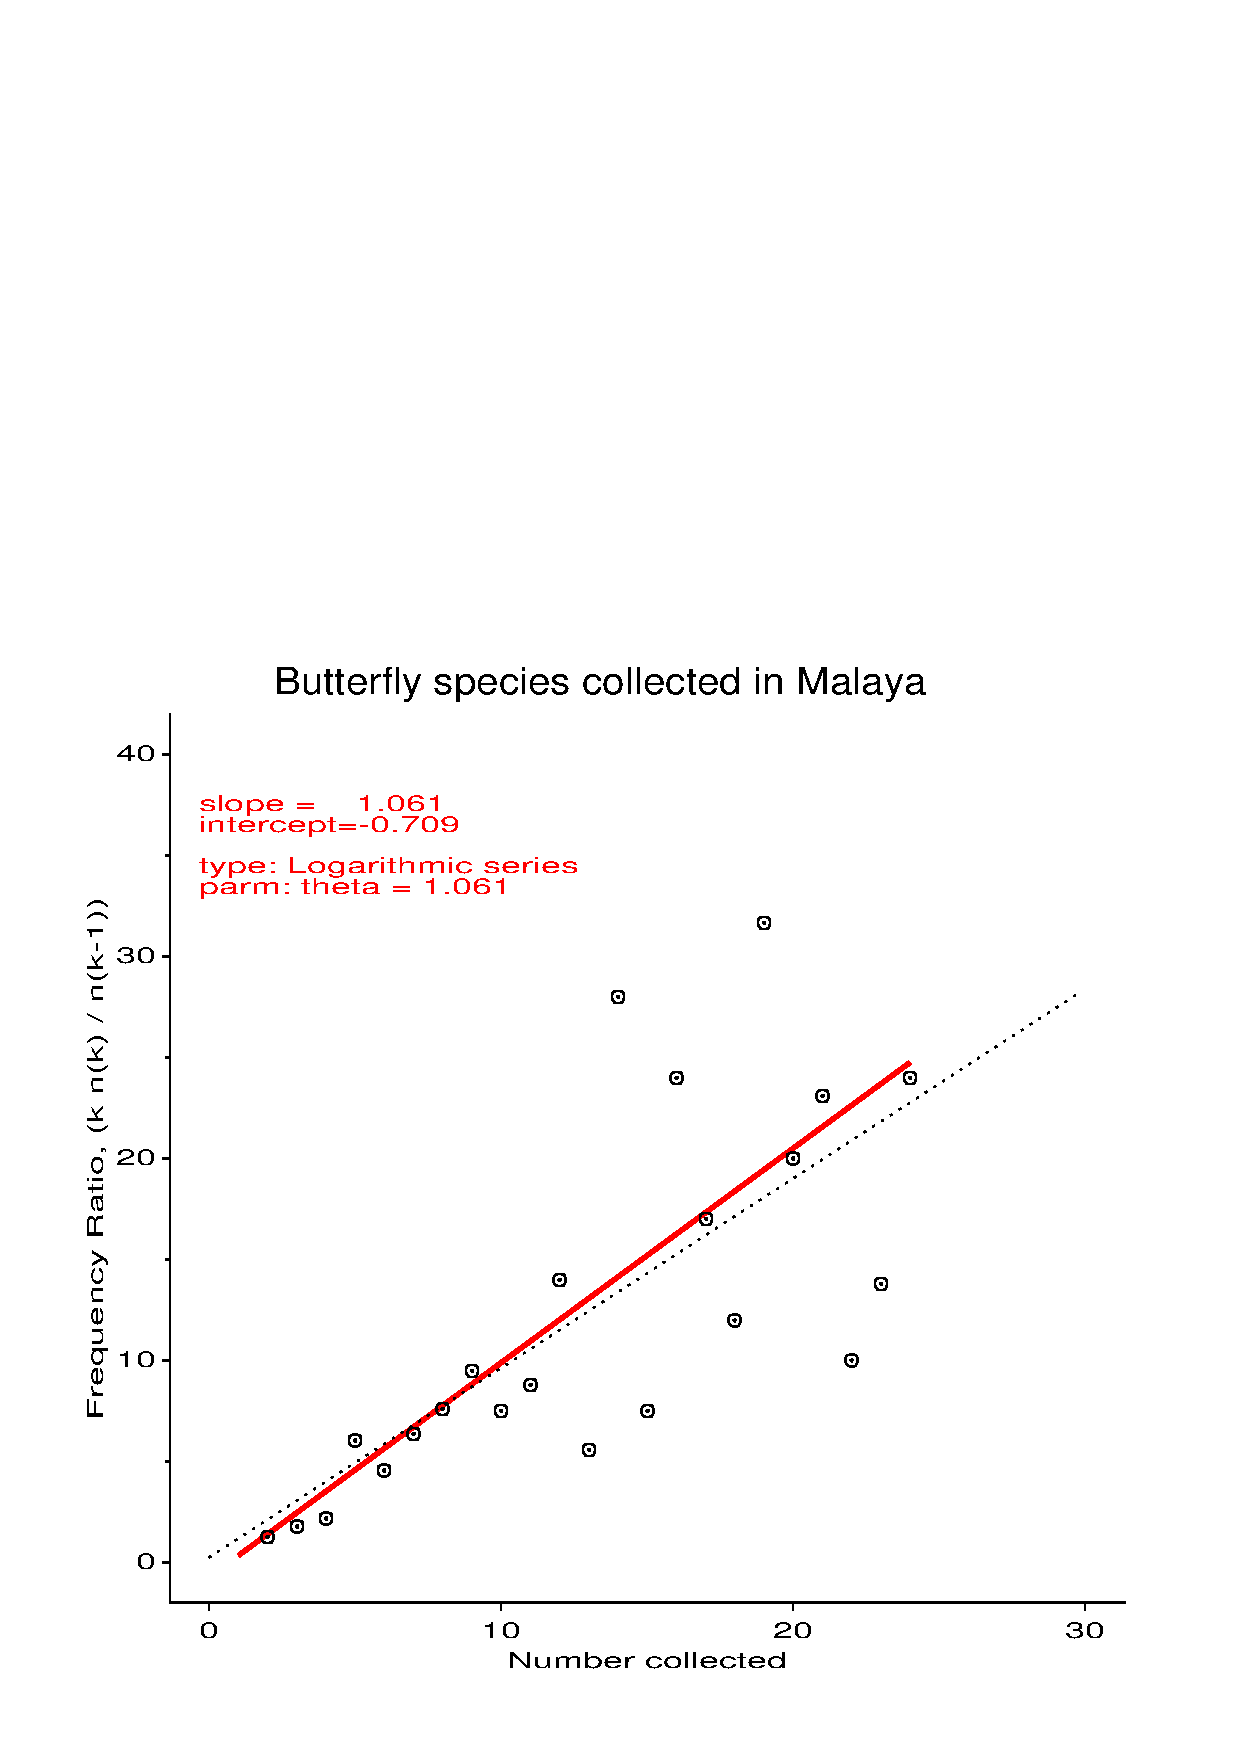
\includegraphics[width=1\linewidth]{orddemo3}\graphicsfile{ch2/fig/orddemo3.eps}{}
 \end{minipage}
 \hfill
 \begin{minipage}[c]{.33\linewidth}
  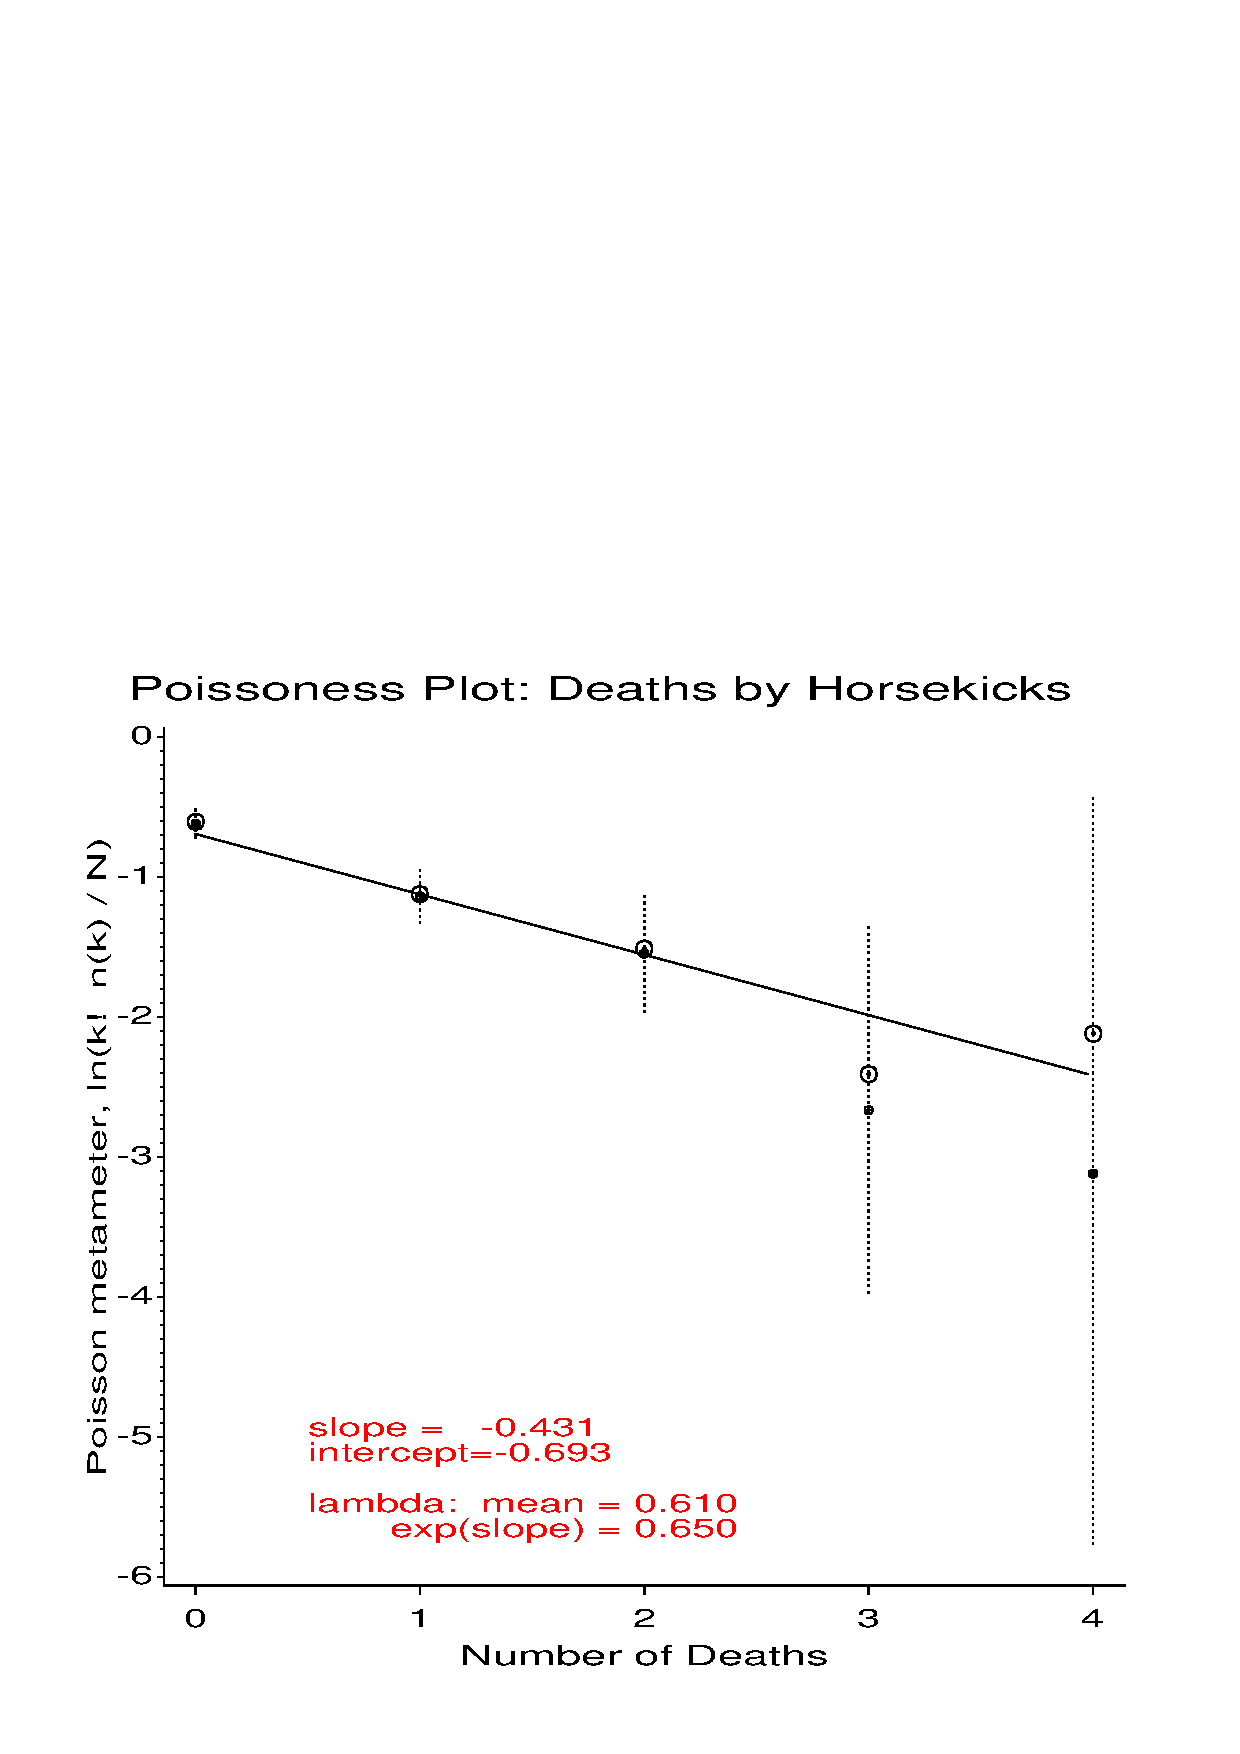
\includegraphics[width=1\linewidth]{poisdemo1}\graphicsfile{ch2/fig/poisdemo1.eps}{}
 \end{minipage}
\end{center}

		% visual table of contents

\chapterprelude{%
Categorical data consist of variables whose values comprise a set
of discrete categories.
Such data require different statistical and graphical methods
than commonly used for quantitative data.
The focus of this book is on visualization techniques and graphical
methods designed to reveal patterns of relationships among
categorical variables. This chapter outlines the basic orientation
of the book and some key distinctions regarding the
analysis and visualization of
categorical data.
}
% \minitoc
% \clearpage


\section{Data visualization and categorical data: Overview}\label{sec:viscat}

\epigraph{Beauty is truth; truth, beauty. \\
  That is all ye know on Earth,
  all ye need to know.}{John Keats, \emph{Ode on a Grecian urn}}


``Data visualization'' can mean many things, from popular press
infographics, to maps of voter turnout or party choice.
Here we use this term in the narrower context of statistical
analysis.  As such, we refer to an approach to data analysis that focuses
on \emph{insightful} graphical display in the service of both
\emph{understanding} our data and \emph{communicating} our results to others.

We may display the raw data, some
summary statistics, or some indicators of the quality or adequacy
of a fitted model.  The word ``insightful'' suggests that the goal
is (hopefully) to reveal some aspects of the data which might not
be perceived, appreciated, or absorbed by other means.
As in the quote from Keats, the overall
aims include both beauty and truth, though each of these are
only as perceived by the beholder.

Methods for visualizing quantitative data have a long history
and are now widely used in both data analysis and in data presentation, and
in both popular and scientific media.
Graphical methods for categorical data,
however, have only a more recent history, and are consequently
not as widely used.  The goal of this book is to show concretely how
data visualization may be usefully applied to categorical data.

``Categorical'' means different things in different
contexts.  We introduce the topic in \secref{sec:whatis}
with some examples illustrating
\begin{seriate}
\item types of categorical variables: binary, nominal, and ordinal,
\item data in case form vs.\ frequency form,
\item frequency data vs.\ count data,
\item univariate, bivariate, and multivariate data, and
\item the distinction between explanatory and response variables.
\end{seriate}

Statistical methods for the analysis of categorical data also fall into two
quite different categories, described and illustrated in \secref{sec:strategies}:
\begin{seriate}
\item the simple randomization-based
methods typified by
the classical Pearson chi-squared ($\chi^2$) test, Fisher's exact test, 
and Cochran-Mantel-Haenszel
tests, and
\item the model-based methods represented by
logistic regression, \loglin, and generalized linear models.
\end{seriate}
In this book, \chrange{ch:discrete}{ch:corresp}
are mostly related to the randomization-based methods;
\chrange{ch:logistic}{ch:loglin}
illustrate the model-based methods.

In \secref{sec:methods} we describe some important similarities
and
differences between categorical data and
quantitative data, and discuss the implications of these differences for
visualization techniques.
\secref{sec:vis} outlines a strategy of data analysis
focused on visualization.

In a few cases we show \R code or results as illustrations here,
but the fuller discussion of using \R for categorical data
analysis is postponed to \chref{ch:working}.


\section{What is categorical data?}\label{sec:whatis}

A \term{categorical variable} is one for which the possible measured
or assigned values
consist of a discrete set of categories, which may be \emph{ordered} or
\emph{unordered}.
Some typical examples are:
\begin{itemize*}
\item \var{Gender}, with categories ``Male'', ``Female''.
\item \var{Marital status}, with categories ``Never married'', ``Married'',
``Separated'', ``Divorced'', ``Widowed''.
\item \var{Fielding position} (in baseball), with categories
``Pitcher'', ``Catcher'', ``1st base'', ``2nd base'',  $\dots$, ``Left field''.
\item \var{Side effects} (in a pharmacological study), with categories
``None'', ``Skin rash'', ``Sleep disorder'', ``Anxiety'', $\dots$.
\item \var{Political attitude}, with categories ``Left'', ``Center'', ``Right''.
\item \var{Party preference} (in Canada), with categories ``NDP'', ``Liberal'', ``Conservative'', ``Green''.
\item \var{Treatment outcome}, with categories ``no improvement'', ``some
improvement'', or ``marked improvement''.
\item \var{Age}, with categories ``0-9'', ``10-19'', ``20-29'', ``30-39'',
$\dots$ .
\item \var{Number of children}, with categories $0, 1, 2, \dots$ .
\end{itemize*}

As these examples suggest, categorical variables differ in the number of
categories: we often distinguish
\term{binary variables} (or \term{dichotomous variables}) such as \var{Gender}
from those with more than two categories (called \term{polytomous variables}).
For example, \tabref{tab:berk220} gives data on $4,526$ applicants
to graduate departments at the University of California at Berkeley
in 1973, classified by two binary variables, gender and admission status.
\ixe{Berkeley admissions}
\begin{table}[htb]
\caption{Admissions to Berkeley graduate programs}
\label{tab:berk220}
 \begin{center}
\begin{tabular}{lrr|r}
\hline
  & Admitted & Rejected & Total  \\
\hline
 Males & 1198 & 1493 & 2691  \\
 Females & 557 & 1278 & 1835  \\
\hline
 Total & 1755 & 2771 & 4526  \\
\hline
\end{tabular}
\end{center}
\end{table}

Some categorical variables (\var{Political attitude}, \var{Treatment outcome})
may have ordered categories (and are called \term{ordinal}),
while other (\term{nominal}) variables like \var{Marital status}
have unordered categories.%
\footnote{An ordinal variable may be defined as one whose categories are
\emph{unambiguously} ordered along a \emph{single} underlying dimension.
Both marital status and fielding position may be weakly ordered, but
not on a single dimension, and not unambiguously.}
For example, \tabref{tab:arthrit0} shows a $2 \times 2 \times 3$ table of
ordered outcomes (``none'', ``some'' or ``marked'' improvement)
to an active treatment for rheumatoid
arthritis compared to a placebo for men and women.
\ixe{Arthritis treatment}
\begin{table}[tb]

\caption{Arthritis treatment data}\label{tab:arthrit0}
\begin{center}
\begin{tabular}{ll|rrr|r}
\hline
     &  & \multicolumn{3}{c|}{Improvement}            &  \\
\hline
   Treatment&  Sex    &None    &Some    &Marked  &  Total \\[1ex]
\hline
   Active   &  Female &      6 &      5 &     16 &     27 \\
            &  Male   &      7 &      2 &      5 &     14 \\ [0.5ex]
%\hline
   Placebo  &  Female &     19 &      7 &      6 &     32 \\
            &  Male   &     10 &      0 &      1 &     11 \\[1ex]
\hline
   Total    &         &     42 &     14 &     28 &     84 \\
\hline
\end{tabular}
\end{center}
\end{table}



Finally, such variables differ in the
fineness or level to which some underlying observation has been
categorized for a particular purpose.
From one point of view, \emph{all} data
may be considered categorical because the precision of measurement
is necessarily finite, or an inherently continuous variable may be recorded only to limited precision.

But this view is not helpful for the applied
researcher because it neglects the phrase ``for a particular purpose''.
Age, for example, might be treated as a quantitative variable in a study of native language vocabulary, or as an ordered categorical variable
with decade groups (0-10, 11-20, 20-30, $\dots$)
in terms of
the efficacy or side-effects of treatment for depression, or even as a
binary variable (``child'' vs.\  ``adult'') in an analysis of survival following an epidemic or natural disaster. In the analysis of
data using categorical methods, continuous variables are often recoded
into ordered categories with a small set of categories for some purpose.%
\footnote{
This may be a waste of information available in the original
variable, and should be done for substantive reasons, not mere
convenience.  For example, some researchers unfamiliar with
regression methods often perform a ``median-split'' on
quantitative predictors
so they can use ANOVA methods. Doing this precludes the possibility
of determining if those variables have non-linear relations with
the outcome while also decreasing statistical power.
}

\subsection{Case form vs.\ frequency form}\label{sec:case-freq}
In many circumstances, data is recorded on each individual or experimental
unit.  Data in this form is called case data,
or data in \term{case form}.
The data in \tabref{tab:arthrit0}, for example, were derived from
the individual data listed in the data set \data{Arthritis}
from the \Rpackage{vcd}.  The following lines show the first
five  of $N=84$ cases in the \data{Arthritis} data,
\begin{knitrout}
\definecolor{shadecolor}{rgb}{1, 0.961, 0.933}\color{fgcolor}\begin{kframe}
\begin{verbatim}
  ID Treatment  Sex Age Improved
1 57   Treated Male  27     Some
2 46   Treated Male  29     None
3 77   Treated Male  30     None
4 17   Treated Male  32   Marked
5 36   Treated Male  46   Marked
\end{verbatim}
\end{kframe}
\end{knitrout}

Whether or not the data variables, and the questions we ask, call for
categorical or quantitative data analysis,
when the data are in case form,
we can always trace
any observation back to its individual identifier or data record
(for example, if the case with \code{ID} equal to 57 turns out to be unusual
or noteworthy).

Data in \term{frequency form}
has already been tabulated, by counting over the categories of the
table variables. The same data shown as a table in
\tabref{tab:arthrit0} appear in frequency form as shown below.
\begin{knitrout}
\definecolor{shadecolor}{rgb}{1, 0.961, 0.933}\color{fgcolor}\begin{kframe}
\begin{verbatim}
   Treatment    Sex Improved Freq
1    Placebo Female     None   19
2    Treated Female     None    6
3    Placebo   Male     None   10
4    Treated   Male     None    7
5    Placebo Female     Some    7
6    Treated Female     Some    5
7    Placebo   Male     Some    0
8    Treated   Male     Some    2
9    Placebo Female   Marked    6
10   Treated Female   Marked   16
11   Placebo   Male   Marked    1
12   Treated   Male   Marked    5
\end{verbatim}
\end{kframe}
\end{knitrout}

Data in frequency form may be analyzed by methods
for quantitative data if there is a quantitative response variable
(weighting each group by the cell frequency, with a weight
variable).
Otherwise, such data are generally
best analyzed by methods for categorical data, where
statistical models are often expressed as models for the
frequency variable, in the form of an \R formula
like \verb|Freq ~ .|.

In any case, an observation in a data set in
frequency form refers
to all cases in the cell collectively, and these cannot be identified individually.
Data in case form can always be reduced to frequency form,
but the reverse is rarely possible. In \chref{ch:working},
we identify a third format, \term{table form}, which is the
\R representation of a table like \tabref{tab:arthrit0}.

\subsection{Frequency data vs.\ count data}\label{sec:freq-count}
In many cases the observations representing the classifications of events (or variables) are
recorded from \emph{operationally independent} experimental units or individuals, typically
a sample from some population.  The tabulated data may be called
\term{frequency data}.  The data in \tabref{tab:berk220} and \tabref{tab:arthrit0}
are both examples of frequency data because each tabulated observation 
comes from a different person.

However, if several events or variables are observed for the same units or individuals, those events are not
operationally independent, and it is useful to use the term
\term{count data} in this situation.  These terms (following
\citet{Lindsey:95}) are by no means standard, but
the distinction is often important, particularly in statistical
models for categorical data.

For example, in a tabulation of the number of male
children within families (\tabref{tab:saxdata}, described in
\secref{sec:uni-multi} below),
the number of male children in a given family would be a \emph{count} variable,
taking values $0, 1, 2, \dots$.  The number of independent families with
a given number of male children is a \emph{frequency} variable.
Count data also arise when we tabulate a sequence of events over time
or under different circumstances in a number of individuals.

\ixe{Families in Saxony}
\begin{table}[htb]
 \caption{Number of Males in 6115 Saxony Families of Size 12}\label{tab:saxdata}
 \begin{center}
 \begin{tabular}{lrrrrrrrrrrrrr}
  \hline
  Males & 0 & 1 & 2 & 3 & 4 & 5 & 6 & 7 & 8 & 9 & 10 & 11 & 12 \\ 
  Families & ~~~3 & ~~24 & ~104 & ~286 & ~670 & 1033 & 1343 & 1112 & ~829 & ~478 & 181 & ~~45 & ~~~7 \\ 
  \hline
 \end{tabular}
 \end{center}
\end{table}


\subsection{Univariate, bivariate, and multivariate data}\label{sec:uni-multi}
Another distinction concerns the number of variables: one, two or
(potentially) many shown in a data set or table, or used in some
analysis.
\tabref{tab:berk220} is an example of a bivariate (two-way) \ctab
and \tabref{tab:arthrit0} classifies the observations by three variables.
Yet, we will see later
that the Berkeley admissions data also recorded
the department to which potential students applied (giving a three-way
table), and in the arthritis data, the age of subjects was also
recorded.

Any \ctab (in frequency or table form) therefore records the \emph{marginal totals}, summed over all
variables not represented in the table.
For data in case form, this means simply ignoring (or not recording)
one or more variables;  the ``observations'' remain the same.
Data in frequency form, however, result in smaller tables when
any variable is ignored;  the ``observations'' are the cells of
the \ctab. For example, in the \data{Arthritis} data, ignoring \var{Sex}
gives the smaller $2 \times 3$ table for \var{Treatment} and \var{Improved}.
\begin{knitrout}
\definecolor{shadecolor}{rgb}{1, 0.961, 0.933}\color{fgcolor}\begin{kframe}
\begin{verbatim}
  Treatment Improved Freq
1   Placebo     None   29
2   Treated     None   13
3   Placebo     Some    7
4   Treated     Some    7
5   Placebo   Marked    7
6   Treated   Marked   21
\end{verbatim}
\end{kframe}
\end{knitrout}


In the limiting case, only one table variable may be recorded or
available, giving the categorical equivalent of univariate data.
For example, \tabref{tab:saxdata} gives data on the distribution
of the number of male children in families with 12 children
(discussed further in \exref{ex:saxony1}).
These data were part of a large tabulation of the sex distribution
of families in Saxony in the 19$^{th}$ century, but the data in \tabref{tab:saxdata}
have only one discrete classification variable, number of males.
Without further information, the only statistical questions concern
the form of the distribution.
We discuss methods for fitting and graphing such discrete distributions
in \chref{ch:discrete}.
The remaining chapters relate to bivariate and multivariate data.
\ixe{Families in Saxony}


\subsection{Explanatory vs.\ Response variables}\label{sec:exp-resp}
\ix{variable!response \~|(}
Most statistical models make a distinction between \term{response variables}
(or \emph{dependent}, or \emph{criterion} variables)
and
\term{explanatory variables}
(or \emph{independent}, or \emph{predictor} variables).

In the standard (classical) linear models for regression and analysis of variance
(ANOVA), for instance, we treat one (or more) variables as responses,
to be explained by the other, explanatory variables.
The explanatory variables may be quantitative or categorical
(e.g., factors in \R).
This affects only the details of how the model is specified
or how coefficients are interpreted for
\func{lm} or \func{glm}.  In these classical models,
the response variable (``treatment outcome'', for example), must be
considered quantitative,  and the model attempts to describe how the
\emph{mean} of the distribution of responses changes with the values
or levels of the explanatory variables, such as age or gender.

When the response variable is categorical, however, the standard linear
models do not apply, because they assume a normal (Gaussian) distribution
for the model residuals.  For example, in \tabref{tab:arthrit0}
the response variable
is \var{Improvement}, and even if numerical scores were assigned
to the categories ``none'', ``some'', ``marked'', it may be unlikely
that the assumptions of the classical linear models could be met.

Hence, a categorical \emph{response} variable generally requires analysis
using methods for categorical data, but categorical \emph{explanatory} variables
may be readily handled by either method.

The distinction between response and explanatory variables also
becomes important in the use of \loglin models for frequency tables
(described in \chref{ch:loglin}), where models can be specified
in a simpler way (as equivalent logit models) by focusing on the response
variable.
\ix{variable!response \~|)}


\section{Strategies for categorical data analysis}\label{sec:strategies}

Data analysis typically begins with exploratory and graphical methods designed
to expose features of the data, followed by statistical analysis
designed to summarize results, answer questions and draw conclusions.
Statistical methods for the analysis of categorical data can be classified into two
broad categories:
those concerned with \emph{hypothesis testing} per se versus those concerned with \emph{model building}.

%\DONE{DM: What about explorative analysis? MF: edited above}

\subsection{Hypothesis testing approaches}\label{sec:strategies-hyp}
In many studies, the questions of substantive interest translate readily
into questions concerning hypotheses about \term{association} between variables, a more general idea than that of correlation
(\emph{linear} association) for quantitative variables.
If a non-zero association exists, we may wish to characterize the
strength of the association numerically and understand the pattern or
nature of the association.

For example, in \tabref{tab:berk220}, a main question is:
``Is there evidence of gender-bias in admission to graduate school?''
Another way to frame this: ``Are males more likely to be admitted?''
These questions can
be expressed in terms of an association between gender and
admission status in a $2 \times 2$ \ctab\
of applicants classified by these two variables.
If there is evidence for an association, we can assess its strength by a variety of
measures, including the difference in proportions admitted for men
and women or the ratio of the odds of admission for men compared to
women, as described in \secref{sec:twoway-twobytwo}.

Similarly, in \tabref{tab:arthrit0}, questions about the efficacy of the
treatment for rheumatoid arthritis can be answered in terms of
hypotheses about the associations among the table variables:
\var{Treatment}, \var{Sex}, and the \var{Improvement} categories.
Although the main concern might be focused on the overall association between
\var{Treatment} and \var{Improvement}, one would also wish to know if this association
is the same for men and women.
A \term{stratified analysis} (\secref{sec:twoway-strat}) controls for the effects of background
variables like Sex, and tests for \term{homogeneity of association}
helping to determine if these associations are equal.

Questions involving tests of such hypotheses are answered most easily
using a large variety of specific statistical tests, often based on
randomization arguments.
These include the familiar Pearson chi-squared test for two-way tables,
the Cochran-Mantel-Haenszel test statistics, Fisher's exact test, and a wide range of measures of strength of association.
These tests make minimal assumptions, principally requiring that subjects
or experimental units have been randomly assigned to the categories of
experimental factors.  The hypothesis testing approach is illustrated
in \chref{ch:twoway}--\ref{ch:corresp}, though the emphasis is on graphical
methods which help to understand the nature of association between
variables.

\begin{Example}[haireye0]{Hair color and eye color}
%\begin{table}[htb]

\caption{Hair-color eye-color data}\label{tab:hairdat}
\begin{center}
\begin{tabular}{|lrrrr|r|}
\hline
        & \multicolumn{4}{c|}{Hair Color}        & \\
Eye     &         &         &         &         &       \\
Color   &  Black  &  Brown  &    Red  &  Blond  & Total \\[2ex] \hline
Green   &      5  &     29  &     14  &     16  &    64 \\
Hazel   &     15  &     54  &     14  &     10  &    93 \\
Blue    &     20  &     84  &     17  &     94  &   215 \\
Brown   &     68  &    119  &     26  &      7  &   220 \\[1ex] \hline
Total   &    108  &    286  &     71  &    127  &   592 \\ \hline
\end{tabular}
\end{center}
\end{table}


%\tabref{tab:hairdat}
The data set \data{HairEye} below
records data on the relationship between hair color and eye color
in a sample of nearly 600 students.
\begin{knitrout}
\definecolor{shadecolor}{rgb}{1, 0.961, 0.933}\color{fgcolor}\begin{kframe}
\begin{verbatim}
       Eye
Hair    Brown Blue Hazel Green
  Black    68   20    15     5
  Brown   119   84    54    29
  Red      26   17    14    14
  Blond     7   94    10    16
\end{verbatim}
\end{kframe}
\end{knitrout}

The standard analysis (with \func{chisq.test} or \func{assocstats})
gives a
Pearson \(\chi^2\) of 138.3 with nine degrees of freedom,
indicating substantial departure from independence.  Among the measures of
strength of association, \term{Cramer's V}, $V = \sqrt{\chi^2 / N \min(r-1,c-1)} = 0.279$,
indicates a substantial relationship between hair and eye color.%
\footnote{Cramer's V varies from 0 (no association) to 1 (perfect association).}


% \TODO{DM: Add thresholds for the statistics, at least to the help page
% - when is a relation considered ``substantial''?}

\begin{knitrout}
\definecolor{shadecolor}{rgb}{1, 0.961, 0.933}\color{fgcolor}\begin{kframe}
\begin{verbatim}
                    X^2 df P(> X^2)
Likelihood Ratio 146.44  9        0
Pearson          138.29  9        0

Phi-Coefficient   : 0.483 
Contingency Coeff.: 0.435 
Cramer's V        : 0.279 
\end{verbatim}
\end{kframe}
\end{knitrout}
The further (and perhaps more interesting question) is how do we
understand the \emph{nature} of this association between hair
and eye color?
Two graphical methods related to the hypothesis testing approach
are shown in \figref{fig:haireye02}.

\begin{knitrout}
\definecolor{shadecolor}{rgb}{1, 0.961, 0.933}\color{fgcolor}\begin{figure}[!htbp]

\centerline{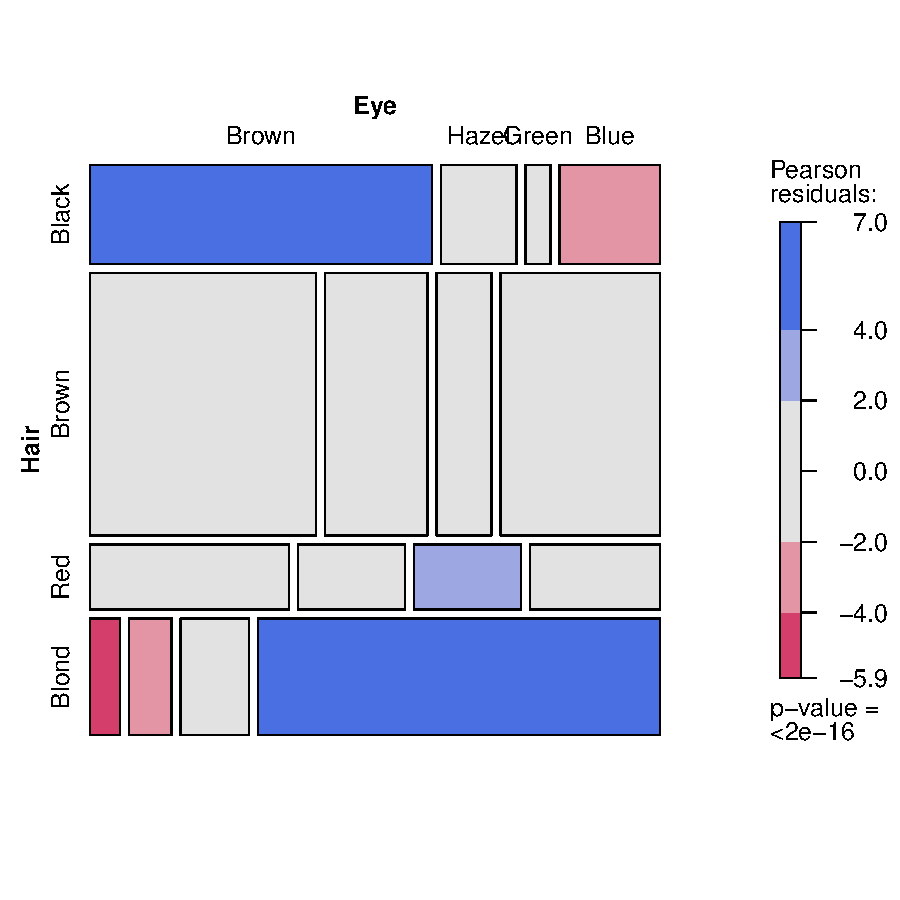
\includegraphics[width=.49\textwidth]{ch01/fig/haireye02-1} 
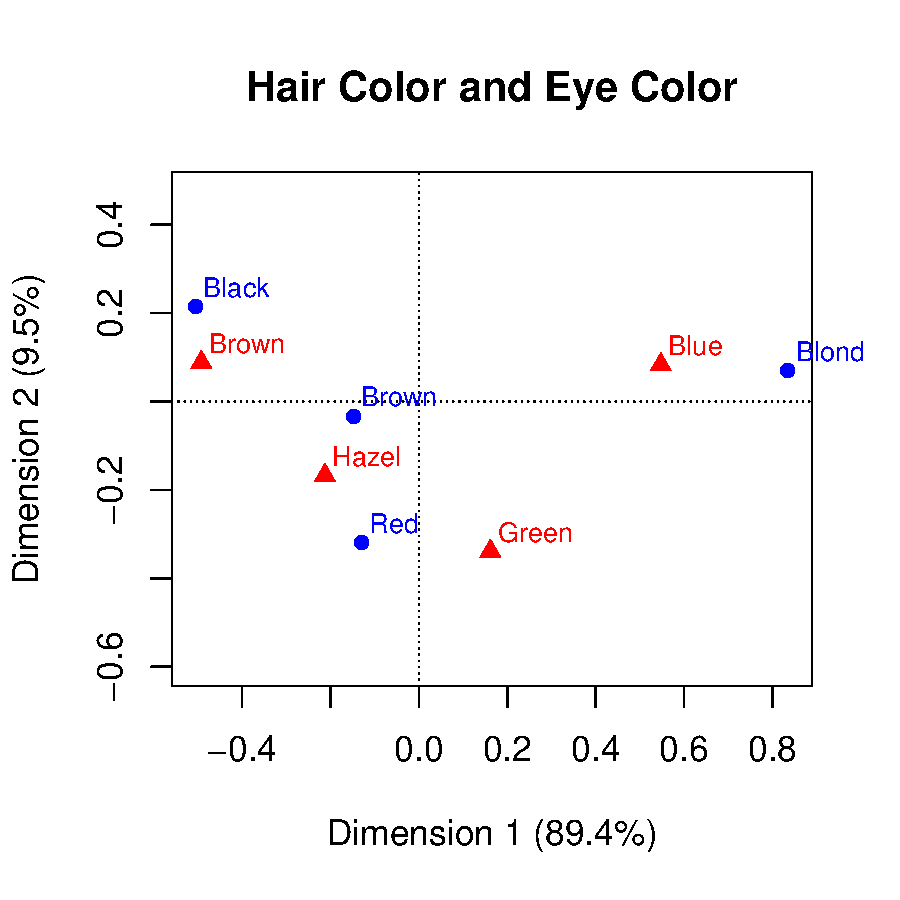
\includegraphics[width=.49\textwidth]{ch01/fig/haireye02-2} }

\caption[Graphical displays for the hair color and eye color data]{Graphical displays for the hair color and eye color data. Left: mosaic display; right: correspondence analysis plot\label{fig:haireye02}}
\end{figure}


\end{knitrout}
The left panel of \figref{fig:haireye02} is a \term{mosaic display}
(\chref{ch:mosaic}), constructed so that the size of each rectangle
is proportional to the observed cell frequency. The shading
reflects the cell contribution to the \(\chi^2\) statistic---shades of blue
when the observed frequency is substantially greater than the
expected frequency under independence, shades of red when the observed frequency
is substantially less, as shown in the legend.

The right panel of this figure shows the results of
a \ca (\chref{ch:corresp}), where the deviations of the hair color and eye
color points from the origin accounts for as much of the \(\chi^2\)
as possible in two dimensions.

We observe that both the hair colors and the eye colors
are ordered from dark to light in the mosaic display and along
Dimension 1 in the \ca plot.  The deviations between observed
and expected frequencies have an opposite-corner pattern in the
mosaic display, except for the combination of red hair and green
eyes, which also stand out as the largest values on Dimension 2
in the \CA plot.
Displays such as these provide a means to understand \emph{how}
the variables are related.
\end{Example}

\subsection{Model building approaches}
Model-based methods provide tests of equivalent
hypotheses about associations, but
offer additional advantages (at the cost of additional assumptions)
not provided by the simpler hypotheses-testing approaches.
Among these advantages, model-based methods provide estimates,
standard errors and confidence intervals for parameters, and the
ability to obtain predicted (fitted/expected) values with associated measures
of precision.

We illustrate this approach here for a dichotomous response variable,
where it is often convenient to
construct a model relating a function of the probability, $\pi$,
of one event to a linear combination of the explanatory variables.
Logistic regression uses the \term{logit function},
\begin{equation*}
 \logit ( \pi ) \equiv \log_e \left( \frac { \pi } {1 - \pi} \right)
\end{equation*}
which may be interpreted as the \term{log odds} of the given event.
A linear logistic model
can then be expressed as
\begin{equation*}
 \logit ( \pi ) = \beta_0 + \beta_1 x_1 + \beta_2 x_2 + \dots
\end{equation*}

Statistical inferences from model-based methods provide tests of
hypotheses for the effects of the predictors, $x_1, x_2, \dots$,
but they also provide estimates of parameters in the model,
$\beta_1, \beta_2, \dots$ and associated confidence intervals.
Standard modeling tools allow us to graphically display the
fitted response surface (with confidence or prediction intervals)
and even to extrapolate these predictions beyond the given data.
A particular advantage of the logit representation
in the logistic regression model is that estimates of odds ratios
(\secref{sec:twoway-twobytwo})
may be obtained directly from the parameter estimates.

\begin{Example}[nasa0]{Space shuttle disaster}
\ixd{Space shuttle disaster|(}
To illustrate the model-based approach,
the graph in \figref{fig:spaceshuttle0} is based on
a logistic regression model predicting the probability of a
failure in one of the O-ring seals used in the 24 NASA space shuttles
prior to the disastrous launch of the
\emph{Challenger} in January, 1986.  The explanatory variable is the ambient temperature (in Fahrenheit) at the time of the flight.
The sad story behind these data, and the lessons to be learned for
graphical data display are related in \exref{ex:nasa}.

\begin{knitrout}
\definecolor{shadecolor}{rgb}{1, 0.961, 0.933}\color{fgcolor}\begin{figure}[!htbp]

\centerline{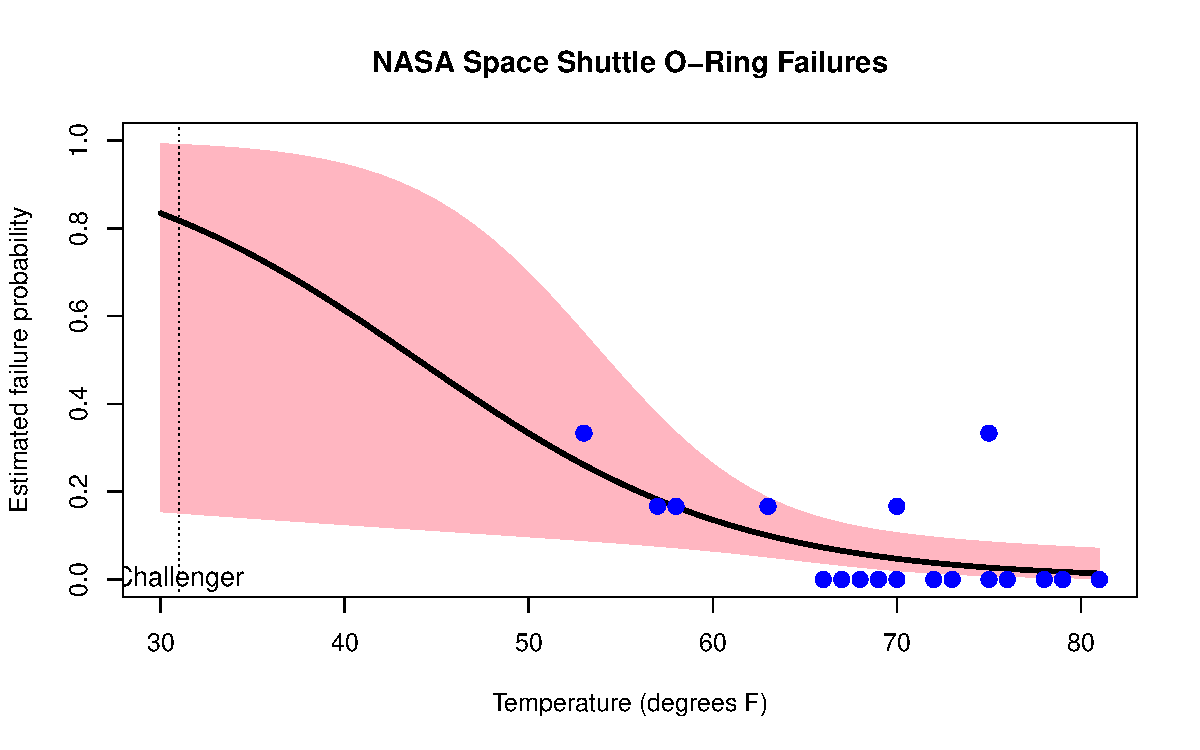
\includegraphics[width=.7\textwidth]{ch01/fig/spaceshuttle0-1} }

\caption[Space shuttle O-ring failure, observed and predicted probabilities]{Space shuttle O-ring failure, observed and predicted probabilities. The dotted vertical line at \degree{31} shows the prediction for the launch of the \emph{Challenger}.\label{fig:spaceshuttle0}}
\end{figure}


\end{knitrout}

Here, we simply note that the fitted model, shown by the solid line in
\figref{fig:spaceshuttle0}, corresponds to the prediction equation
(with standard errors shown in parentheses),
\begin{equation*}
 \logit ( \mbox{Failure} ) =  \cwe{5.09}{3.06} - \cwe{0.116}{0.047} \mbox{ Temperature}
 \end{equation*}%
A hypothesis test that failure probability is unassociated with temperature
is equivalent to the test that the coefficient for temperature in this
model equals 0; this test has a $p$-value of 0.014, convincing evidence
for rejection.

The parameter estimate for temperature, $-0.116$, however, gives more information.  Each \degree{1} increase in temperature decreases the log odds
of failure by 0.116, with 95\% confidence interval $\left[-0.208,
-0.0235\right]$.  The equivalent odds ratio is $\exp(-0.116) = 0.891$ $\left[0.812, 0.977\right]$.
Equivalently, a \degree{10} \emph{decrease} in temperature corresponds to
an odds ratio of a failure of
$\exp(10 \times 0.116) = 3.18$, more than tripling the odds of a failure.

When the \emph{Challenger} was launched, the temperature was only \degree{31}.
The shaded region in \figref{fig:spaceshuttle0} show 95\% prediction intervals
for failure probability.  All previous shuttles (shown by the points
in the figure) had been launched at much warmer temperatures, so the
prediction interval (the dashed vertical line)
at \degree{31} represents a considerable extrapolation
beyond the available data.  Nonetheless, the model building approach
does provide such predictions along with measures of their uncertainty.
\figref{fig:spaceshuttle0} is a graph
that might have saved lives.

\ixd{Space shuttle disaster|)}
\end{Example}

%\TODO{Perhaps replace this example with a similar one for the \code{Donner} data}

% \TODO{DM: Remove Donner party example to shorten up the intro? One example
% for logistig regression seems enough here.}

\begin{Example}[donner0]{Donner Party}
In April--May of 1846 (three years before the California gold rush),
the Donner and Reed families set out for California from the American mid-west
in a wagon train to seek a new life and perhaps their fortune in the new
American frontier.
By mid July, a large group had reached a site
in present-day Wyoming;  George Donner was elected to lead what was
to be called the ``Donner Party,'' which eventually numbered 87 people
in 23 wagons, along with their oxen, cattle, horses, and worldly possessions.

They were determined to reach California as quickly as possible.
Lansford Hastings, a self-proclaimed trailblazer (retrospectively,
of dubious distinction), proposed that the party follow him through
a shorter path through the Wasatch Mountains.  Their choice
of ``Hastings's Cutoff'' proved disastrous: Hastings had never
actually crossed that route himself, and the winter of of 1846 was to
be one of the worst on record.

In October, 1846, heavy snow stranded them in the eastern Sierra
Nevada, just to the east of a pass which bears their name today.
The party made numerous attempts to seek rescue, most turned back
by blizzard conditions. Relief parties in March--April 1847 rescued
40, but discovered grizzly evidence that those who survived had
cannibalized those who died.

Here we briefly examine of how statistical models and
graphical evidence can shed light on the question of
who survived in the Donner party.

\begin{knitrout}
\definecolor{shadecolor}{rgb}{1, 0.961, 0.933}\color{fgcolor}\begin{figure}[!htbp]

\centerline{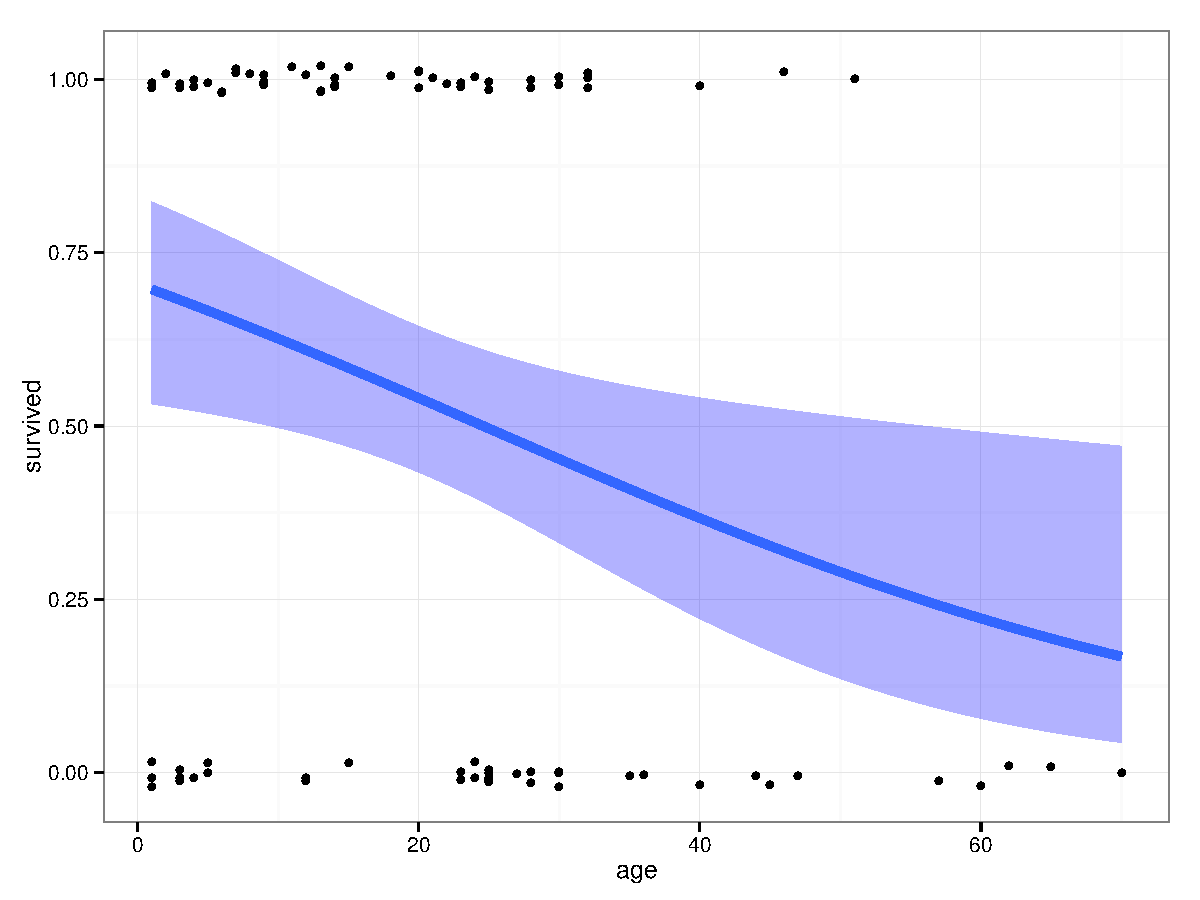
\includegraphics[width=.7\textwidth]{ch01/fig/donner0-1} }

\caption[Donner party data, showing the relationship between age and survival]{Donner party data, showing the relationship between age and survival. The blue curve and confidence band give the predicted probability of survival from a linear logistic regression model.\label{fig:donner0}}
\end{figure}


\end{knitrout}

\figref{fig:donner0} is an example of what we call a \emph{data-centric, model-based}
graph of a discrete (binary) outcome: lived (1) versus died (0). That is, it shows
both the data and a statistical summary based on a fitted statistical model.
The statistical model provides a smoothing of the discrete data.

The jittered points at the top and bottom of the graph show survival in relation
to age of the person.  You can see that there were more people who survived
among the young, and more who died among the old.
The blue curve in the plot shows the fitted probability of survival from
a linear logistic regression model for these data with a 95\% confidence band
for the predictions.  The prediction equation for this model can
be given as:

\begin{equation*}
 \logit ( \mbox{survived} ) =  \cwe{0.868}{0.372} - \cwe{0.0353}{0.015} \mbox{ age}
 \end{equation*}

 The equation above implies that the log odds of survival decreases by 0.0352 with each additional year of
 age or by $10 \times 0.0352 = 0.352$ for an additional decade.
 Another way to say this is that the odds of survival is multiplied by
 $\exp({0.353}) = .702$ with each 10 years of age, a 30\% decrease.

 Of course, these visual and statistical summary depends on the validity of fitted model.
 For contrast, \figref{fig:donner0-other} shows two other model-based smoothers that
 relax the assumption of the linear logistic regression model.
 The left panel shows the result of fitting a semi-parametric model with a
 natural cubic spline with one more degree of freedom than the linear
 logistic model.  The right panel shows the fitted curve for a non-parametric,
 locally weighted scatterplot smoothing (loess) model.  Both of these hint that the relationship of survival to age is
 more complex than what is captured in the linear logistic regression model.
 We return to these data in \chref{ch:logistic}.


\begin{knitrout}
\definecolor{shadecolor}{rgb}{1, 0.961, 0.933}\color{fgcolor}\begin{figure}[!htbp]

\centerline{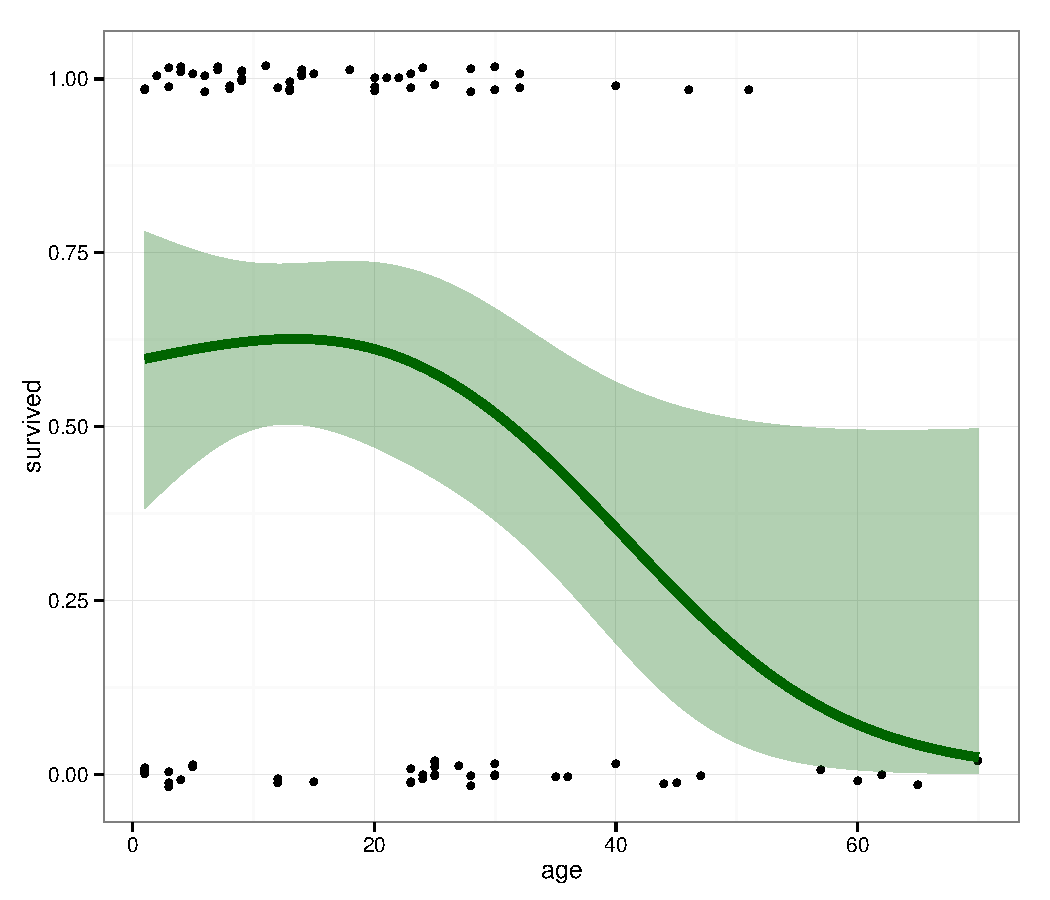
\includegraphics[width=.49\textwidth]{ch01/fig/donner0-other-1} 
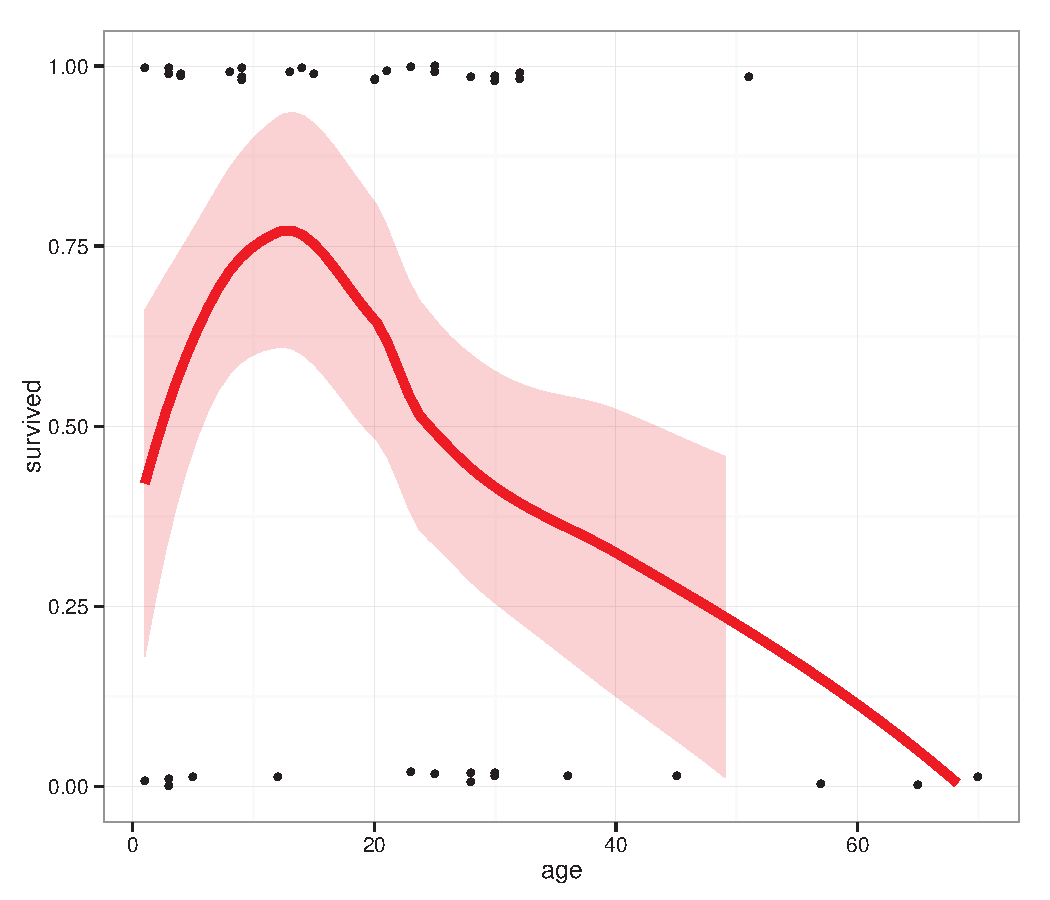
\includegraphics[width=.49\textwidth]{ch01/fig/donner0-other-2} }

\caption[Donner party data, showing other model-based smoothers for the relationship between age and survival]{Donner party data, showing other model-based smoothers for the relationship between age and survival. Left: using a natural spline; right: using a non-parametric loess smoother.\label{fig:donner0-other}}
\end{figure}


\end{knitrout}

%\DONE{Complete this example}
\end{Example}

\section{Graphical methods for categorical data}\label{sec:methods}

\epigraph{You can see a lot, just by looking}{Yogi Berra}

The graphical methods for categorical data described in this book
are in some cases straightforward adaptations of more familiar
visualization techniques developed for quantitative data.
Graphical principles and strategies, and the relations between
the visualization approach and traditional statistical methods
are described in a number of sources, including
\citet{Chambers-etal:83},
\citet{Cleveland:VisData} and several influential books by Tufte
\citep{Tufte:83,Tufte:90,Tufte:97,Tufte:2006}.

The fundamental ideas of statistical graphics as a comprehensive system
of visual signs and symbols with a grammar and semantics was first proposed
in Jacques Bertin's \emph{Semiology of Graphics} \citeyearpar{Bertin:83},
These ideas were later extended to a computational theory
in Wilkinson's \emph{Grammar of Graphics} \citeyearpar{Wilkinson:2005},
and implemented in \R in Hadley Wickham's \Rpackage{ggplot2}
\citep{Wickham:2009:ggplot2,ggplot2}.

Another perspective on visual data display is presented in \secref{sec:intro-goals}
focusing on the communication goals of statistical graphics.
However, the discrete nature of categorical data implies that
some familiar graphic methods need to be adapted, while in other
cases we require a new graphic metaphor for data display.
These issues are illustrated in \secref{sec:intro-catdata}.
\secref{sec:effect-order} discusses the principle of effect ordering
for categorical variables in graphs and tables.

\subsection{Goals and design principles for visual data display}\label{sec:intro-goals}

Designing good graphics is surely an art, but as surely, it is
one that ought to be informed by science.
In constructing a graph, quantitative and qualitative information is
encoded by visual features, such as position, size, texture, symbols
and color. This translation is reversed when a person studies a
graph. The representation of numerical magnitude and categorical
grouping, and the apperception of patterns and their \emph{meaning} must be extracted from the visual display.

There are many views of graphs, of graphical perception, and of
the roles of data visualization in discovering and communicating
information.
On the one hand, one may regard a graphical display as a \emph{stimulus}---
a package of information to be conveyed to an idealized observer.
From this perspective certain questions are of interest:  which
form or graphic aspect promotes greater accuracy or speed of judgment
(for a particular task or question)?  What aspects lead to greatest
memorability or impact?
Cleveland \citep{ClevelandMcGill:84b,ClevelandMcGill:85,Cleveland:93:JCGS},
Spence and Lewandowsky
\citep{LewandowskySpence:89,Spence:90,SpenceLewandowsky:90} have made important contributions to our understanding of
these aspects of graphical display.

An alternative view regards a graphical display as an act
of \emph{communication}---like a narrative, or even a poetic text or work of art.
This perspective places the greatest emphasis on the desired
communication goal, and judges the effectiveness of a graphical
display in how well that goal is achieved \citep{FriendlyKwan:2011}.
\citet{Kosslyn:85,Kosslyn:89} and \citet{Tufte:83,Tufte:90,Tufte:97}
have articulated this perspective most clearly.

In this view,
an effective graphical display, like good writing, requires an
understanding of its \emph{purpose}---what aspects of the data are to be
communicated to the viewer.  In writing we communicate most
effectively when we know our audience and tailor the message
appropriately. So too, we may construct a graph in different ways to:
\begin{seriate}
  \item use ourselves,
  \item present at a conference or meeting of our colleagues,
  \item publish in a research report, or
  \item communicate to a general audience
\end{seriate}
(\citet[Ch. 1]{Friendly:91}, \citet{FriendlyKwan:2011}).
\figref{fig:presentation-exploration} illustrates a basic contrast between graphs
for presentation purposes, designed to appeal persuasively to a large audience
(one-to-many)
and the use of perhaps many graphs we might make for ourselves for
exploratory data analysis (many-to-one).
% \citep{Unwin:99}.

\begin{figure}[htb]
\centering
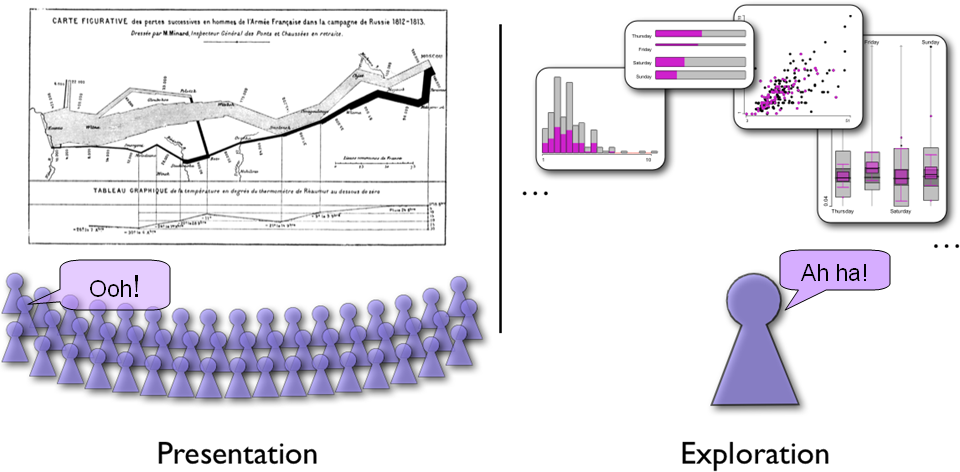
\includegraphics[width=.8\textwidth]{ch01/fig/presentation-exploration2}
\caption[Different communication purposes require different graphs]{Different communication purposes require different graphs. For presentations, a single, carefully crafted graph may appeal best to a large audience; for exploratory analysis, many related images from different perspectives for a narrow audience (often you!). \emph{Source}: Adapted from a blog entry by Martin Theus, \url{http://www.theusrus.de/blog/presentation-vs-exploration/}.}\label{fig:presentation-exploration}
\end{figure}

\figref{fig:datadisp}
shows one organization of visualization methods in terms
of the \emph{primary} use or intended communication goal,
the functional \emph{presentation goal}, and suggested corresponding
\emph{design principles}.
\begin{figure}[htbp]
  \centering
  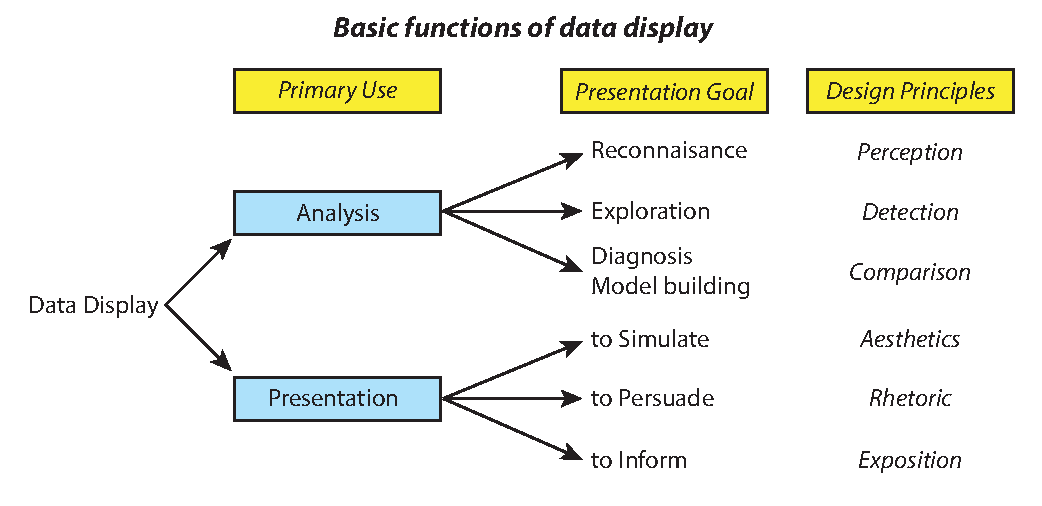
\includegraphics[width=\textwidth]{ch01/fig/datadisp}
  \caption[Basic functions of data display]{A taxonomy of the basic functions of data display by intended use, presentation goal and design principles.}\label{fig:datadisp}
\end{figure}

We illustrate these ideas and distinction in the examples below, most of which
are treated again in later chapters.

\begin{Example}[arrests0]{Racial profiling: Arrests for marijuana possession}
In a case study that will be examined in detail in \chref{ch:logistic} (\exref{ex:arrests}),
the \emph{Toronto Star} newspaper studied a huge data base of arrest records by
Toronto police for indications of possible racial profiling, i.e., differential
treatment of those arrested on the basis of skin color.
They focused on the charge of simple possession of a small amount of marijuana,
for which enforcement procedures allowed police discretion.  An officer could
release an arrestee with a summons (``Form 9'') to appear in court,
or take the person to a police station for questioning (``Form 10'') or
booking (``Form 11.1'') or order the person held in jail for a bail hearing (``Show cause'').

%\TODO{DM: Add frequency table here? Could be easier compared with mosaic plot.  MF: No, not required for this example}

The statistical issue was whether the data on these arrests showed evidence of differential
treatment in relation to skin color, particularly in the treatment of blacks vs. whites,
controlling, of course, for other factors. Statistical tests on these data
(\chisq tests, loglinear models, logistic regression) showed overwhelming evidence of
differential treatment of blacks and whites. However, tables of these results do not
reveal the nature of this association.

\figref{fig:arrests0-mosaic} is an example of
a graph designed for \emph{analysis}--- a mosaic display (\chref{ch:mosaic})
showing the frequencies of those arrested
on this charge by skin color and release type.  The size of each rectangle shows the
frequency and these are shaded in relation to the asociation between skin color and
release--- blue for positive associations (more than expected under independence) to
red for negative associations.
\begin{figure}[htb]
\centering
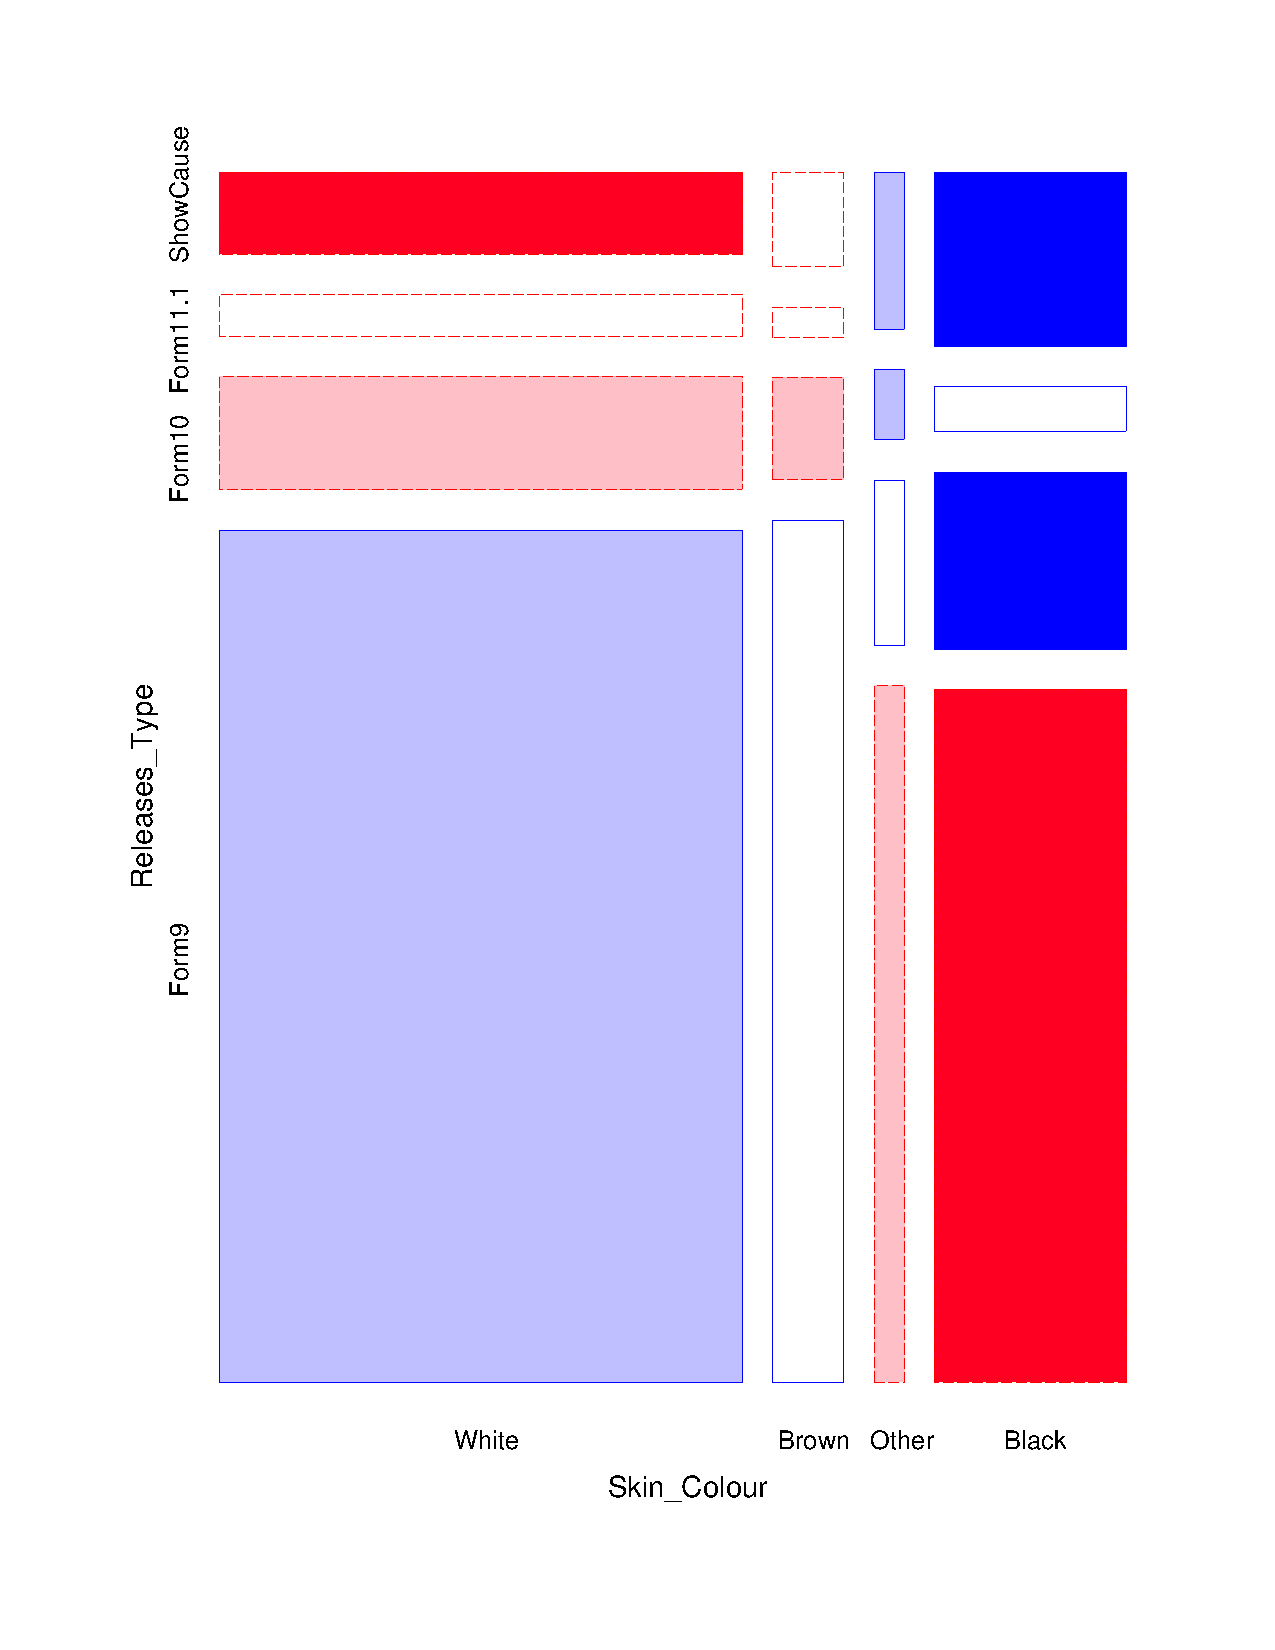
\includegraphics[width=.5\textwidth]{ch01/fig/arrests-skin-color}
\caption{Mosaic display showing the relationship between skin color and release type for those arrested on a charge of simple possession of marijuana in Toronto, 1996-2002.}\label{fig:arrests0-mosaic}
\end{figure}

Once you know how to read such graphs, the pattern is clear: blacks were indeed more likely
to be held for more severe treatment, whites were more likely to be released with a
summons.  But this is hardly a graph that would be clear to a general audience,
and would require a good deal of explanation.

In contrast, \figref{fig:arrests0-star} shows a redesign of this as a \emph{presentation graphic}
prepared by the \emph{Star} and published on December 11, 2002
in conjunction with a meeting between the newspaper and the Toronto Police Services Board
to consider the issue of racial profiling.  The police vehemently denied that racial profiling
was taking place.  The revision makes the point immediately obvious and compelling in the
following ways:
\begin{itemize*}
 \item It announces the conclusion in the figure title: ``Same charge, different treatment''
 \item The text box at the top provides the context for this conclusion
 \item Skin colors ``Brown'' and ``Other'', which were of low frequency were removed,
 and the release categories ``Form 10'' and ``Form 11.1'' were combined as ``released at station.''
 \item The graphic is still a mosaic display, however, it now shows explicitly the number
 of charges laid against whites and blacks and the percentage of each treatment.
 \item The labels for Whites and Blacks were enhanced by indicating what a reader should see for each.
 \item The legend for color is titled non-technically as ``degree of likelihood.''
\end{itemize*}

\begin{figure}[htb]
\centering
%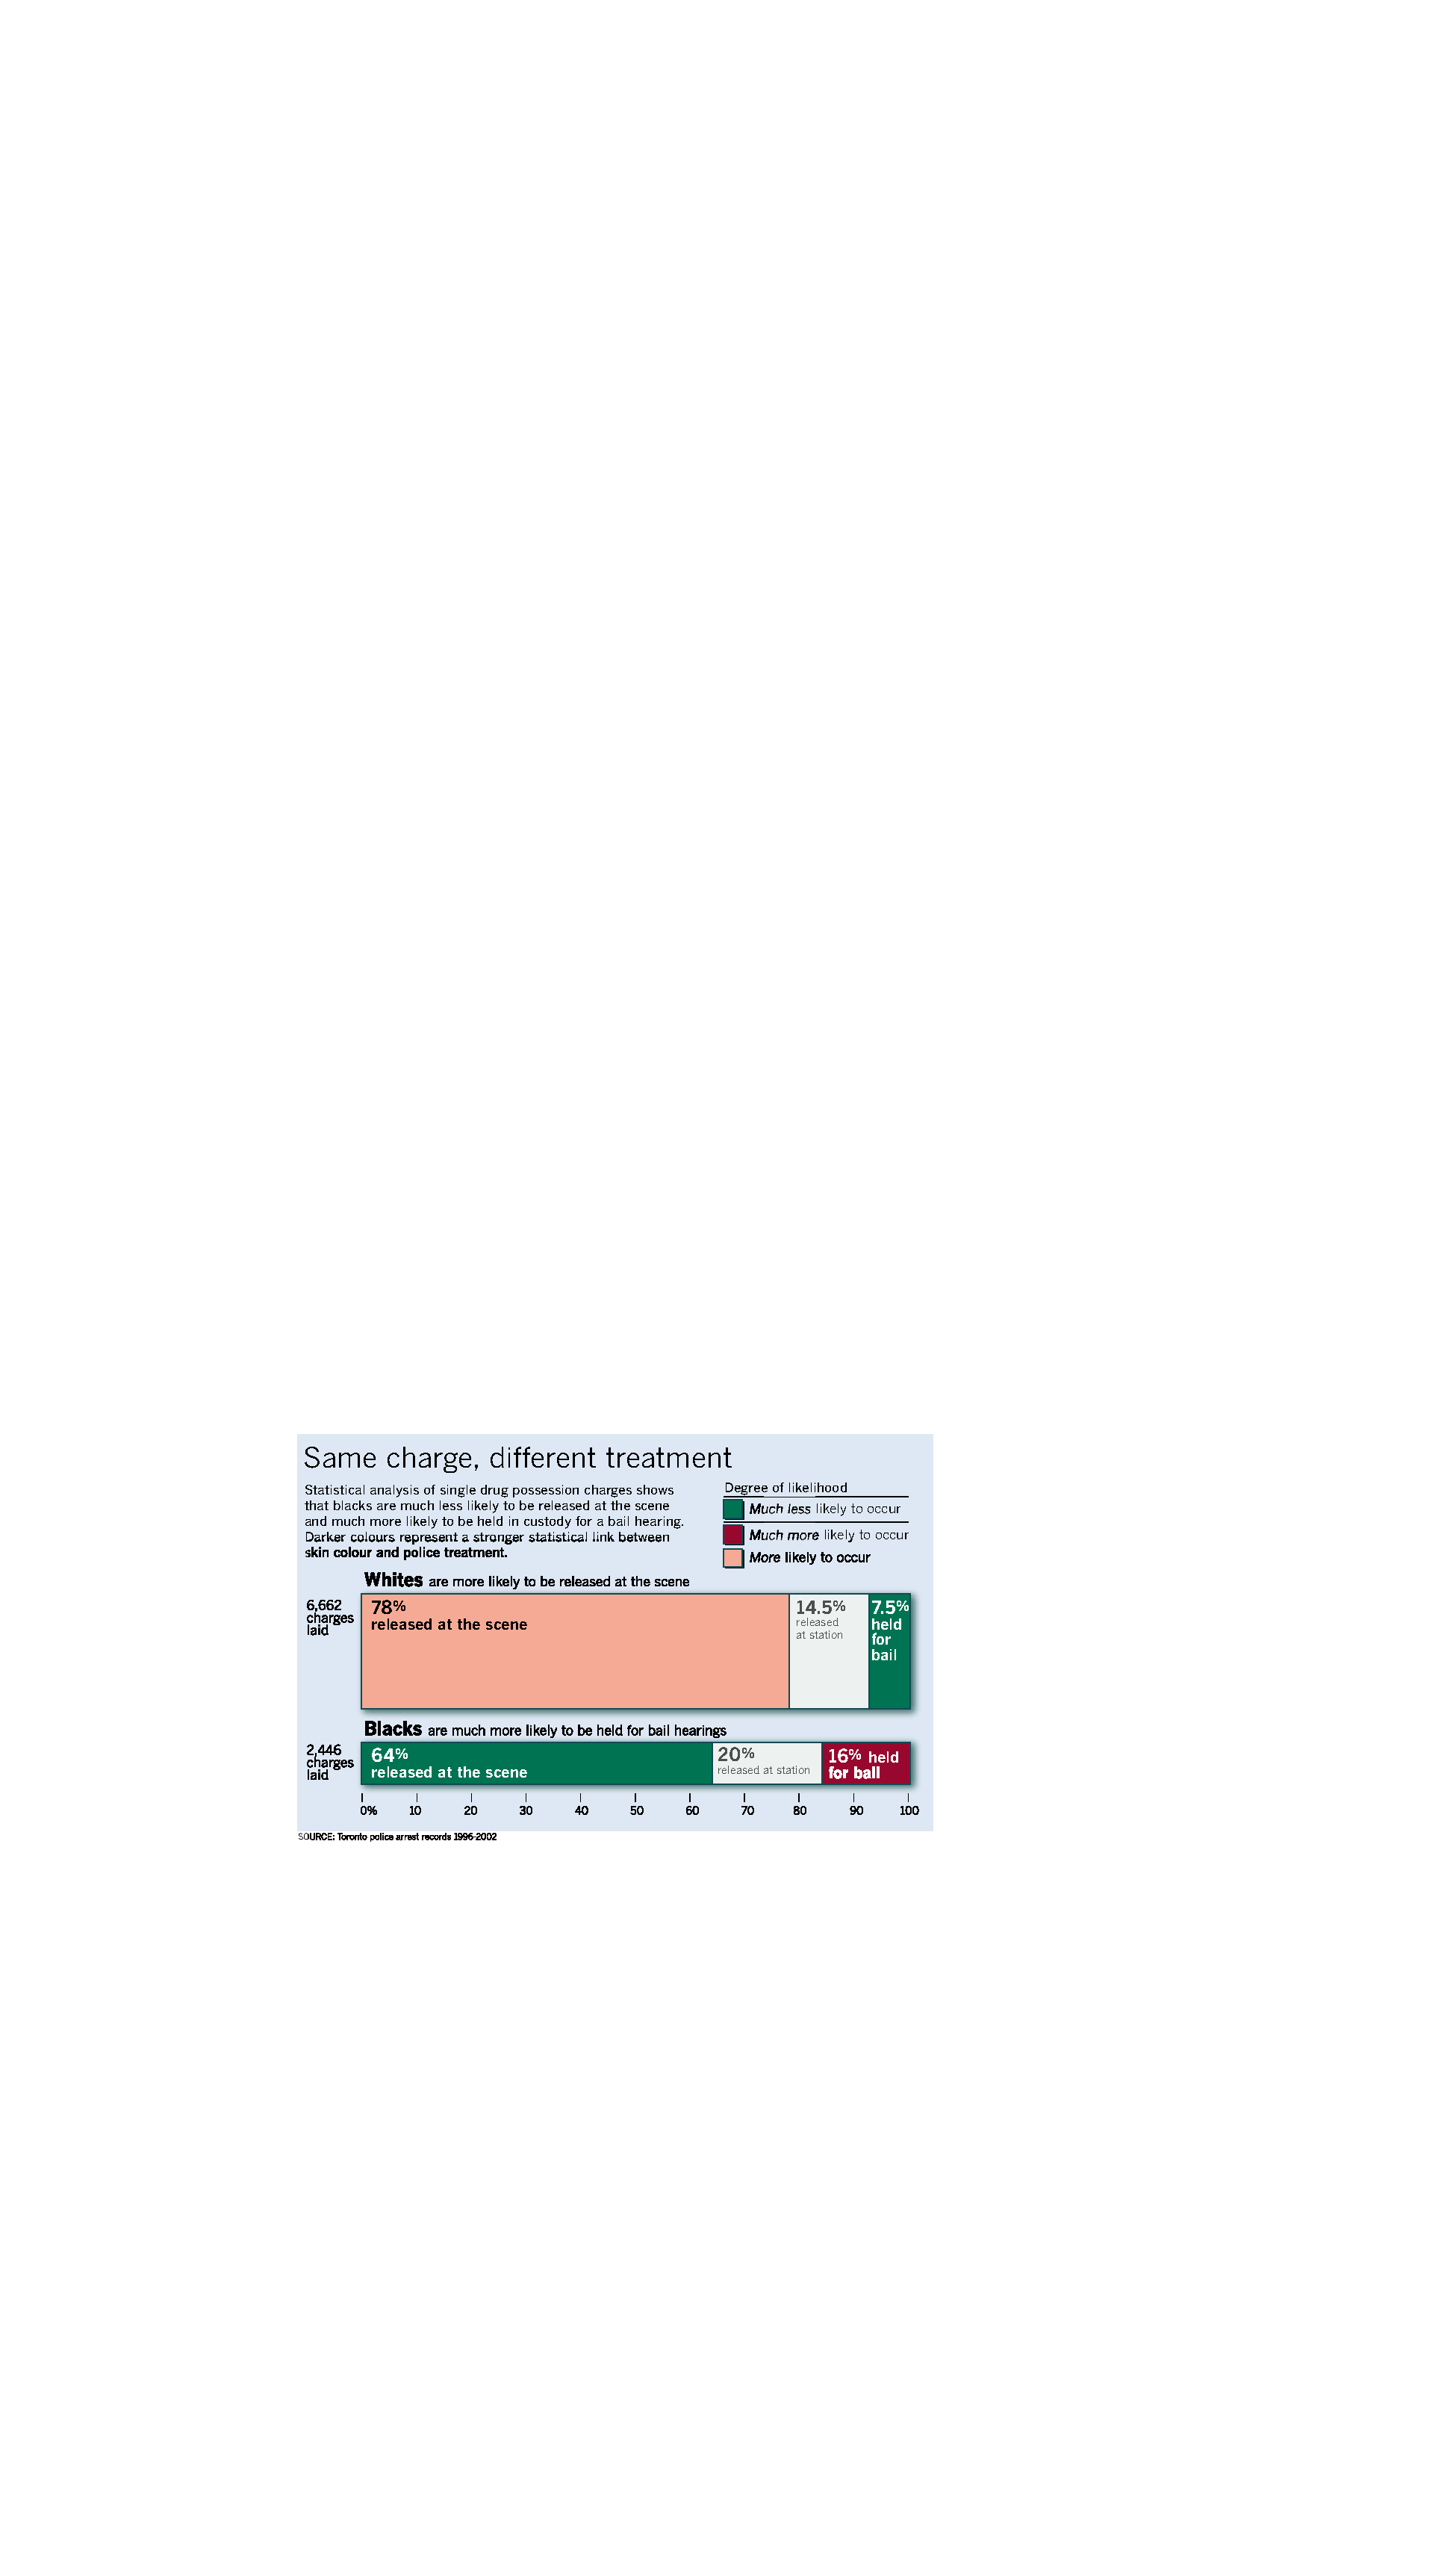
\includegraphics[width=.9\textwidth]{ch01/fig/TorontoStar-graphic-2002-12-11}
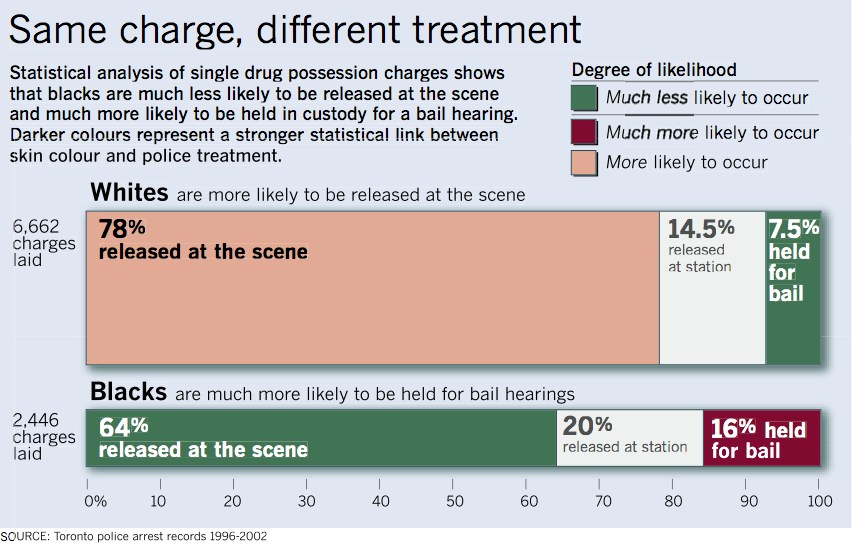
\includegraphics[width=.9\textwidth]{ch01/fig/TorStar/TorontoStar-graphic-2002-12-11-2}
\caption{Redesign of \figref{fig:arrests0-mosaic} as a presentation graphic. \emph{Source}: Graphics department, \emph{The Toronto Star}, December 11, 2002. Used by permission.}\label{fig:arrests0-star}
\end{figure}

Clear communication is not achieved without effort.  The revised graph required several iterations
and emails between the graphic designer and the statistical consultant (the first author of this book)
in the few hours available before the newspaper went to press.
The main question was, ``what are we trying to show here?'' Starting with the original
\figref{fig:arrests0-mosaic} mosaic, we asked ``what can we remove?'' and ``what can we add?''
to make the message clearer.

\end{Example}

% \TODO{Complete this section.  Show a collection of analysis and presentation graphs for categorical data. It is probably better to wait until more chapters are written to provide examples here.}

\subsection{Categorical data require different graphical methods}\label{sec:intro-catdata}

We mentioned earlier, and will see in greater detail
in \chref{ch:logistic} and \chref{ch:loglin},
that statistical models for discrete
response data and for frequency
data are close analogs of the linear regression and ANOVA models
used for quantitative data.
These analogies suggest that the graphical methods
commonly used for quantitative data may be adapted directly to
categorical data.

Happily, it turns out that many of the analysis graphs and diagnostic
displays (e.g., effect plots,
influence plots, added variable and partial residual
plots, etc.)
that have become common adjuncts in the analysis of
quantitative data have been extended to generalized linear models
including logistic regression (\secref{sec:logist-infl})
and \loglin\ models (\secref{sec:glm-diag})
%\DONE{Add forward references to these sections.}

Unhappily, the familiar techniques for displaying raw data are
often disappointing when applied to categorical data.
The simple \scat, for example, widely used to show
the relation between
quantitative response and predictors, when applied to discrete
variables, gives a display of the category combinations,
with all identical values overplotted, and no representation of
their frequency.

Instead, frequencies of categorical variables are often best
represented graphically using \emph{areas} rather than as
position along a scale. \citet{Friendly:95} describes
conceptual and statistical models that give a rationale
for this graphic representation.
\figref{fig:arrests0-mosaic} does this in the form of a
modified bar chart (mosaic plot), where the widths of the horizontal
bars show the proportions of whites and blacks in the data, and
the divisions of each group give the percents of each release type.
Consequently, the areas of each bar are proportional to the
frequency in the cells of this $2 \times 3$ table.

\begin{figure}
  \centering
  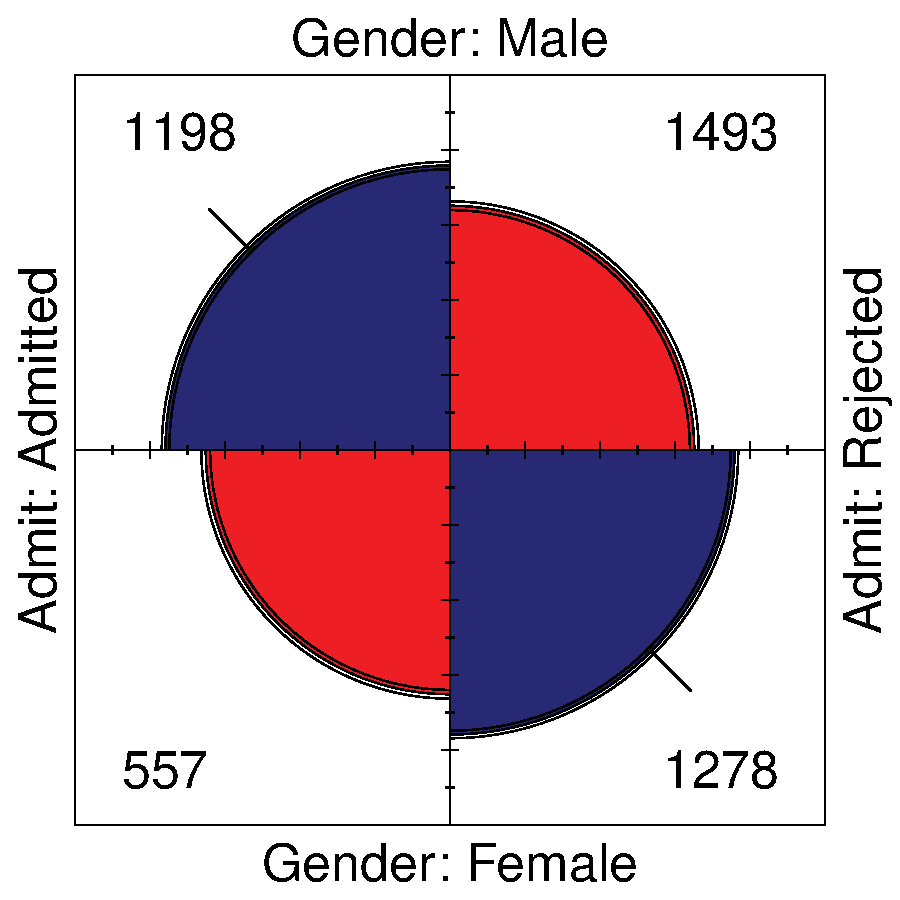
\includegraphics[width=0.49\textwidth]{ch01/fig/berk-fourfold3}
  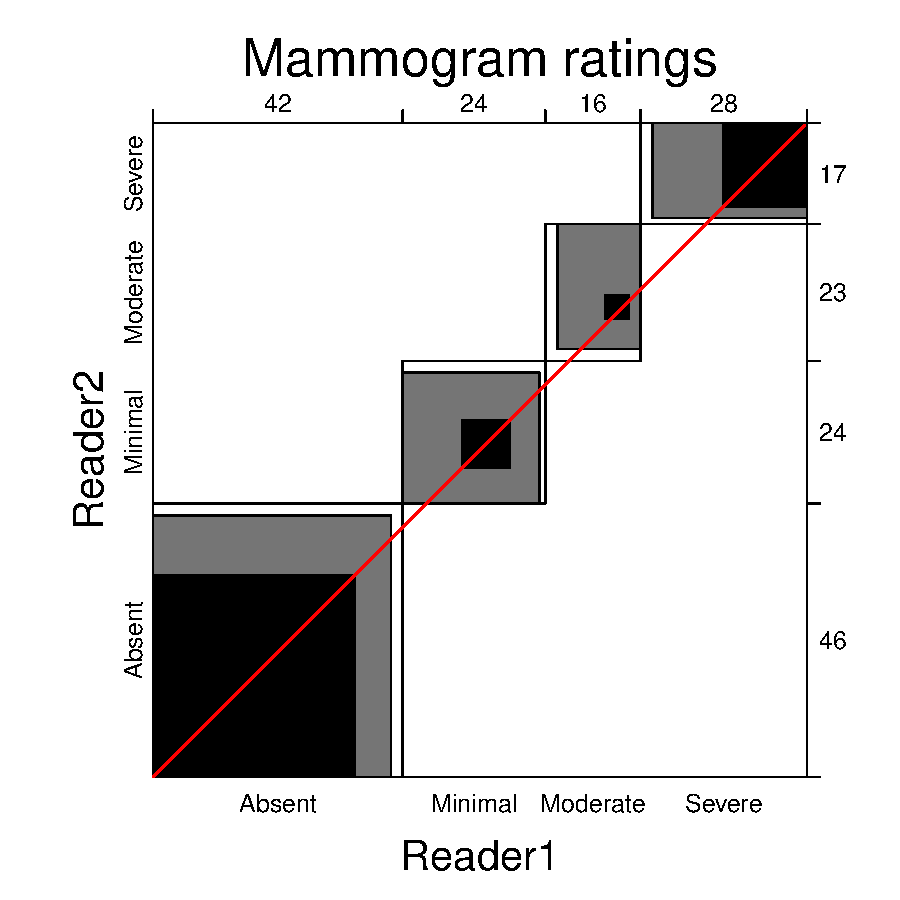
\includegraphics[width=0.49\textwidth]{ch01/fig/mammograms1}
  \caption{Frequencies of categorical variables shown as areas. Left: fourfold display of the relation between gender and admission in the Berkeley data; right: agreement plot for two raters assessing mammograms. }
  \label{fig:area-diagrams}
\end{figure}

As we describe later in this book, using the visual  attribute
\precept{area $\sim$ frequency}
also allows creating novel graphical displays of frequency data
for special circumstances.

\figref{fig:area-diagrams} shows two examples.
The left panel gives a \term{fourfold display} of the frequencies
of admission and gender in the Berkeley data shown in
\tabref{tab:berk220}.
What should be seen at a glance is that males are more often admitted
and females more often rejected (shaded blue); see \secref{sec:twoway-fourfold}
for details.

The right panel shows another specialized display, an \term{agreement chart}
designed to show the strength of agreement in a square table for two raters
(see \secref{sec:twoway-Bangdiwala}).  The example here (\exref{ex:mammograms})
concerns agreement of ratings of breast cancer from mammograms by two raters.
The dark squares along the diagonal show exact agreement; the lighter diagonal
rectangles allow 1-off agreement, and both are shown in relation to chance
agreement (diagonal enclosing rectangles).  What should be seen at a glance
is that exact agreement is moderately strong and extremely strong if you allow
the raters to differ by one rating category.

%\DONE{Complete this section.}

\subsection{Effect ordering and rendering for data display}\label{sec:effect-order}

In plots of quantitative variables, standard methods
(histograms, scatterplots) automatically position values along
ordered scales, facilitating comparison (``which is less/more?'')
and detection of patterns, trends and anomalies.
However, by its nature, categorical data involves discrete variables such as
education level, hair color, geographic region (state or province)
or preference for a political party.
With alphabetic labels for ordered
categories (e.g., education: Low, Medium, High), it is unfortunately all to
easy to end up with a nonsensical display with the categories
ordered High, Low, Medium.  Geographic regions (U.S. states) are often
ordered alphabetically by default as are the names of political parties
and other categorical variables.  This may be useful for lookup, but
for the purposes of comparison
and detection, this is almost always a bad idea.

Instead, \citet{FriendlyKwan:02:effect}, proposed the principle of
\term{effect-order sorting} for visual displays (tables as well as graphs):
% \begin{quote}
% \textbf{sort the data by the effects to be seen to facilitate comparison}
% \end{quote}
\precept{sort the data by the effects to be seen to facilitate comparison}
For quantitative data, this is often achieved by sorting the
data according to means or medians of row and column factors,
called \term{main-effect ordering}.
For categorical data, graphs and tables are often most effective
when the categories are arranged in an order reflecting their
association, called \term{association ordering}.

Another important principle concerns the
\term{rendering} of visual attributes of
elements in graphical displays
\citep{Friendly:02:corrgram}.  For example, categorical variables in plots (and tables)
can be distinguished by any one or more of color, size, shape, or font.
The examples below show the use of color to illustrate the precept:
% \begin{quote}
% \textbf{render the data by the effects to be seen to facilitate detection}
% \end{quote}
\precept{render the data by the effects to be seen to facilitate detection}

\begin{Example}[glass]{British social mobility}
\citet[p. 100]{Bishop-etal:75} analyzed data on the occupations of
3500 British fathers and their sons from a study by \citet{Glass:54},
with five occupational categories:
Professional, Managerial, Supervisory, Skilled manual and Unskilled manual.

One would expect, of course, a strong association between a son's
occupation and that of his father--- the apple doesn't
fall very far from the tree.
Mosaic plots (detailed in \chref{ch:mosaic})
provide a natural way to show such relationships.
\figref{fig:glass-mosaic} shows two such plots.
The left panel shows the result obtained when the table variables
\code{father} and \code{son} are read as factors, and therefore
ordered alphabetically by default.
It is difficult to see any overall pattern, except for the
large values in the diagonal cells (shaded blue) corresponding to equal
occupational status.

\begin{figure}
  \centering
  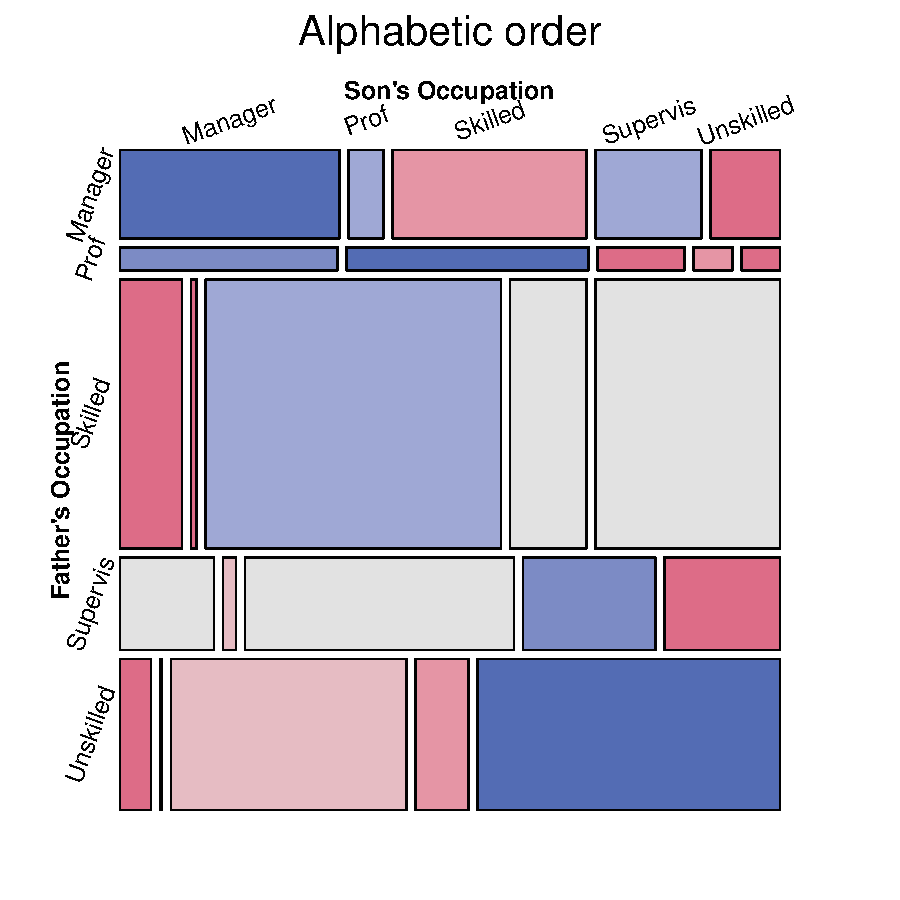
\includegraphics[width=0.49\textwidth]{ch01/fig/glass-mosaic1}
  \hfill
  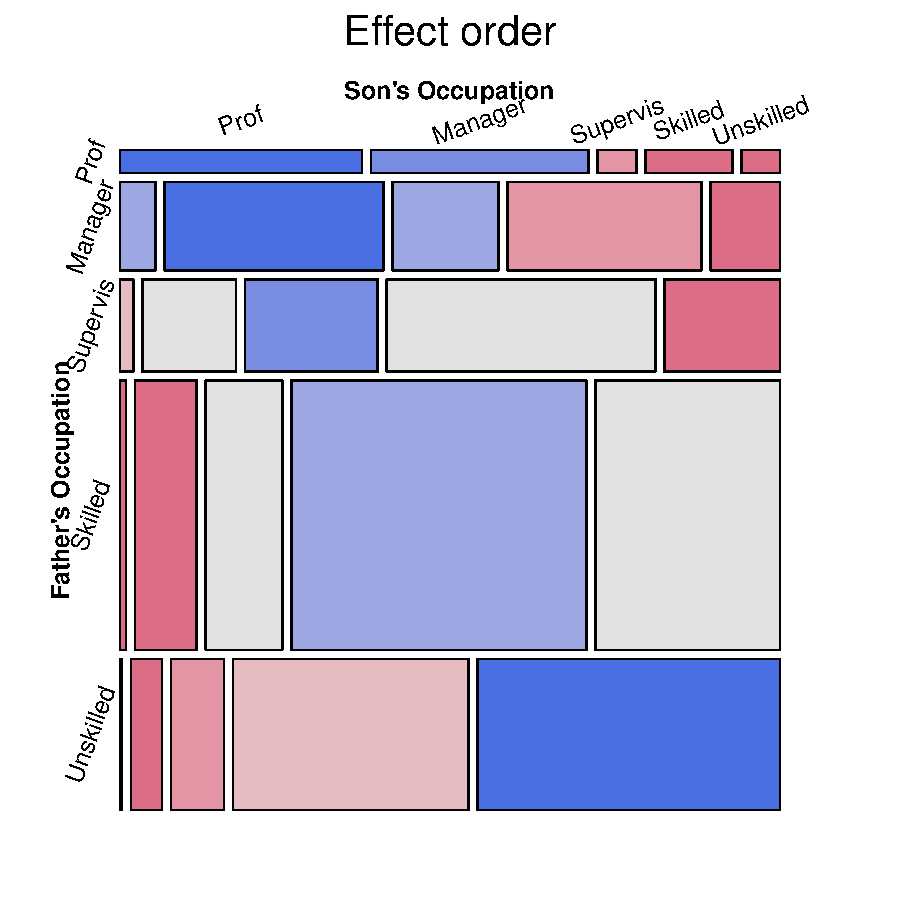
\includegraphics[width=0.49\textwidth]{ch01/fig/glass-mosaic2}
  \caption{Mosaic plots for Glass' mobility table of occupational status.
  In these displays the area of each tile is proportional to frequency
  and shading color shows the departure from independence, using
  blue for positive, red for negative association.
  Left: default alphabetic ordering of categories; right: occupational categories
  ordered by status. 
%   \DONE{PC: The box labels are really overlapping in the effect ordered plot. 
%   Is it possible to change them to be at, say 45 degrees instead of 0 degrees along the x-axis? 
%   UPDATE: I've fixed the code (probably) in ch01/R/glass.R, but can't generate the plot bc I don't have access to the data.}
  }
  \label{fig:glass-mosaic}
\end{figure}
In the right panel, the categories have been arranged in
decreasing order of occupational status to show the
association according to status.
Now you can see a global pattern of shading color, where the
tiles become increasingly red as one moves away from the main
diagonal, reflecting a greater difference between the occupation
of the father and son.
The interpretation here is that most sons remain in their
father's occupational class, but when they differ,
there is little mobility across large steps.

In this example, \code{father} and \code{son} are clearly ordinal
variables and should be treated as such in both graphs and statistical models.
Correspondence analysis (\chref{ch:corresp})
provides a natural way to depict association by assigning scores to
the categories to optimally represent their relationships.
\Loglin models provide special methods
for ordinal variables (\secref{sec:loglin-ordinal})
and square frequency tables (\secref{sec:loglin-square}).

\end{Example}

The ideas of effect ordering and rendering with
color shading to enhance perception can
also be used in tabular displays, as illustrated in the next example.

\begin{Example}[barley]{Barley data}
The classic \data{barley} dataset (in \pkg{lattice})
from \citet{Immer-etal:34}
gives a $10 \times 2 \times 6$ table of yields
of 10 varieties of barley in two years (1931, 1932)
planted at 6 different sites in Minnesota.
\citet{Cleveland:VisData} and many others have used this data to illustrate
graphical methods, and one
surprising finding not revealed in standard tabular displays
is that the data for one site (Morris) may have had
the values for 1931 and 1932 switched.%
\footnote{
This canonical story, like many others in statistics and graphics lore
turns out to be apocryphal on closer examination.
\cite{Wright:2013} recently took a closer look at the original data
and gives an expanded data set as \data{minnesota.barley.yield}
in the \Rpackage{agridat}.  With a wider range of years (1927--1936),
other local effects like weather had a greater impact than the
overall year effects seen in 1931--1932, and the results for the
Morris site no longer stand out as surprising.
}

% This can easily be seen in a dotplot (not shown here)
% of yield by variety, colored by year, and grouped by site.
% The canonical graphical example can be produced
% using \pkg{ggplot2} as follows:

% \DONE{either show graph or remove code.}

% <<barley-dotplot, eval=FALSE>>=
% data(barley, package="lattice")
% library(ggplot2)
% ggplot(data=barley, aes(x=yield, y=variety, color=year)) +
%   geom_point() +
%   facet_wrap(~site)
% @

To focus attention on this suspicious effect in a tabular display,
you can calculate the \emph{yield difference}
$\Delta y_{ij} = y_{ij,1931} - y_{ij,1932}$.
%and arrange these
%in a $10 \times 6$ table as shown below ($i$: varieties, $j$: sites):
%\TODO{This is not correct. FIXME}
% <<barley-diff, eval=FALSE>>=
% yield <- array(barley$yield, c(6, 10, 2))
% dimnames(yield) <- list(
%   site = levels(barley$site),
%   variety = levels(barley$variety),
%   year = levels(barley$year))
% diff <- t(yield[,,2] - yield[,,1])
% @
\tabref{tab:barley2c} shows these values in a $10 \times 6$ table with the rows and columns
sorted by their means (main-effect ordering).  In addition, the table cells
have been colored according to the sign and magnitude of the year difference.
The shading scheme uses blue for large positive values and red for large
negative values, with a white background for intermediate values.
The shading intensity values were determined as
$| \Delta y_{ij} |> \{2, 3\} \times \widehat{\sigma} (\Delta y_{ij} )$.

\definecolor{blueA}{rgb}{0.85,0.85,1}
\definecolor{blueB}{rgb}{0.7 ,0.7 ,1}
\definecolor{redA}{rgb}{1,0.85,0.85} 
\definecolor{redB}{rgb}{1,0.7 ,0.7 } 
%%
%% Table barley2c written by md2tex 17AUG00 17:52
%%
\begin{table}[htb]
 \caption{Barley data, yield differences, 1931-1932, sorted by mean difference, and shaded by value}
 \label{tab:barley2c}
 \begin{center}
  \begin{tabular}{|l|rrrrrr|r|}
   \hline
 & \multicolumn{6}{c|}{\bfseries\large Site   } & \rule{0in}{2.5ex}\\
{\bfseries\large Variety} &  Morris &  Duluth & \brk{University\\Farm} & \brk{Grand\\Rapids} &  Waseca &  Crookston& {\bfseries\large\itshape Mean} \\
   \hline
\multirow{1}*{No. 475} & \cell{redB}{-22} &               6 &              -5 &               4 &               6 & \cell{blueB}{12} &             0.1 \\
\multirow{1}*{Wisconsin No. 38} & \cell{redB}{-18} &               2 &               1 & \cell{blueB}{14} &               1 & \cell{blueB}{14} &             2.4 \\
\multirow{1}*{Velvet} & \cell{redB}{-13} &               4 & \cell{blueB}{13} & \cell{redA}{-9} & \cell{blueB}{13} & \cell{blueA}{9} &             2.9 \\
\multirow{1}*{Peatland} & \cell{redB}{-13} &               1 &               5 & \cell{blueA}{8} & \cell{blueB}{13} & \cell{blueB}{16} &             4.8 \\
\multirow{1}*{Manchuria} & \cell{redA}{-7} & \cell{blueA}{6} &               0 & \cell{blueB}{11} & \cell{blueB}{15} & \cell{blueA}{7} &             5.5 \\
\multirow{1}*{Trebi} &              -3 &               3 & \cell{blueA}{7} & \cell{blueA}{9} & \cell{blueB}{15} &               5 &             6.1 \\
\multirow{1}*{Svansota} & \cell{redA}{-9} &               3 & \cell{blueA}{8} & \cell{blueB}{13} & \cell{blueA}{9} & \cell{blueB}{20} &             7.3 \\
\multirow{1}*{No. 462} & \cell{redB}{-17} &               6 & \cell{blueB}{11} &               5 & \cell{blueB}{21} & \cell{blueB}{18} &             7.4 \\
\multirow{1}*{Glabron} & \cell{redA}{-6} &               4 &               6 & \cell{blueB}{15} & \cell{blueB}{17} & \cell{blueB}{12} &             8.0 \\
\multirow{1}*{No. 457} & \cell{redB}{-15} & \cell{blueB}{11} & \cell{blueB}{17} & \cell{blueB}{13} & \cell{blueB}{16} & \cell{blueB}{11} &             8.8 \\
   \hline
\rule{0in}{2.5ex}{\bfseries\large\itshape Mean} &          -12.2 &             4.6 &             6.3 &             8.2 &            12.5 &            12.5 &             5.3 \\
   \hline
  \end{tabular}
 \end{center}
\end{table}



Effect ordering and color rendering
have the result of revealing a new effect, shown as a regular progression
in the body of the table.
The negative values for Morris now immediately stand out.  In addition,
the largely positive other values show a lower-triangular pattern,
with the size of the yield difference increasing with both row and column means.
Against this background, one other cell, for Velvet grown at Grand Rapids stands out
with an anomalous negative value.

Although the use of color for graphs is now more common in some journals,
color and other rendering details in tables are still difficult.
The published version of \tabref{tab:barley2c} \citep[Table 3]{FriendlyKwan:02:effect}
was forced to use only font shape (normal, italics) to distinguish positive and
negative values.

\end{Example}

Finally, effect ordering is also usefully applied to the variables in multivariate data
sets, which by default, are often ordered in data displays according to their position
in a data frame or alphabetically.
% \TODO{DM: Remove this section if parallel coordinates plots are removed
%   from Sec. 5.7. MF: I'd like to keep this example}

\begin{Example}{Iris data}
The classic \data{iris} data set \citep{Anderson:35,Fisher:36}
gives the measurements in centimeters of the variables sepal length and width and petal length and width, respectively, for 50 flowers from each of 3 species of iris, \emph{Iris setosa}, \emph{versicolor}, and \emph{virginica}.
Such multivariate data are often displayed in \term{parallel coordinate plot}s, using a separate vertical axis for
each variable, scaled from its minimum to maximum.

The default plot, with variables shown in their data frame order is shown in the left panel of \figref{fig:iris-parallel},
and gives rise to the epithet \emph{spaghetti plot} for such displays because of the large number of line crossings.
This feature arises because one variable, sepal width, has negative relations in the species means with the other
variables. Simple rearrangement of the variables to put sepal width last (or first)
makes the relations among the species and the variables more apparent, as shown in the right panel of \figref{fig:iris-parallel}.  This plot has also been enhanced by using \term{alpha-blending} (partial transparency) of thicker
lines, so that the density of lines is more apparent.

\begin{knitrout}
\definecolor{shadecolor}{rgb}{1, 0.961, 0.933}\color{fgcolor}\begin{figure}[!htbp]

\centerline{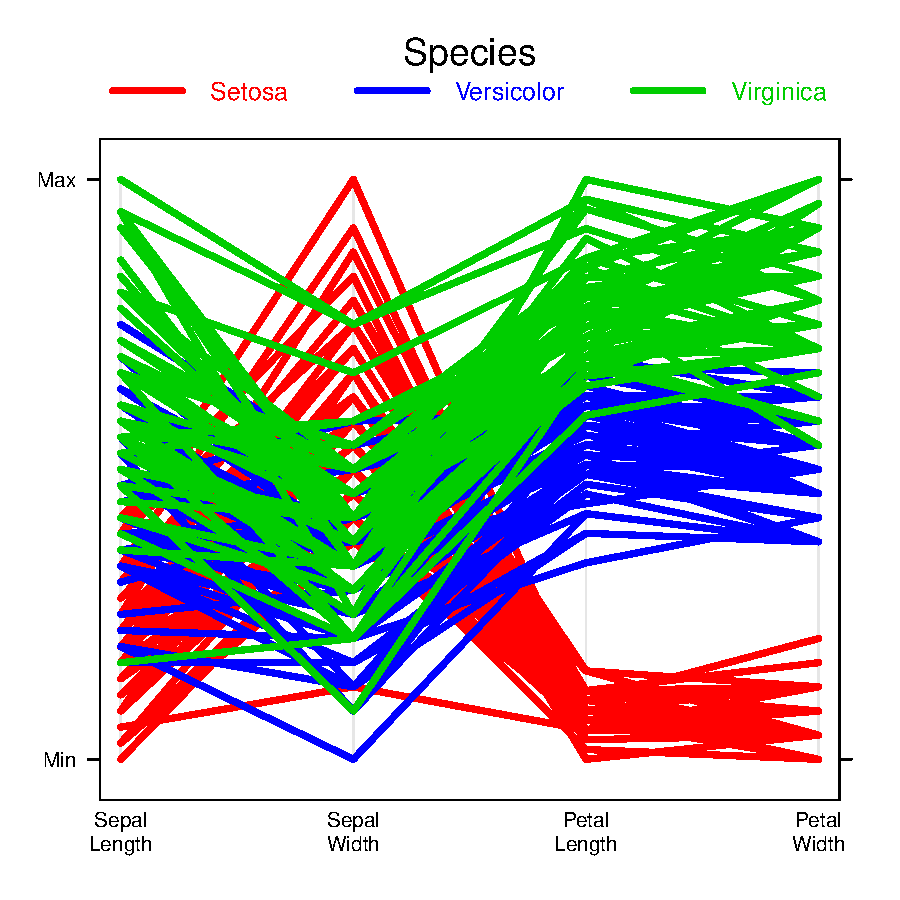
\includegraphics[width=.49\textwidth]{ch01/fig/iris-parallel-1} 
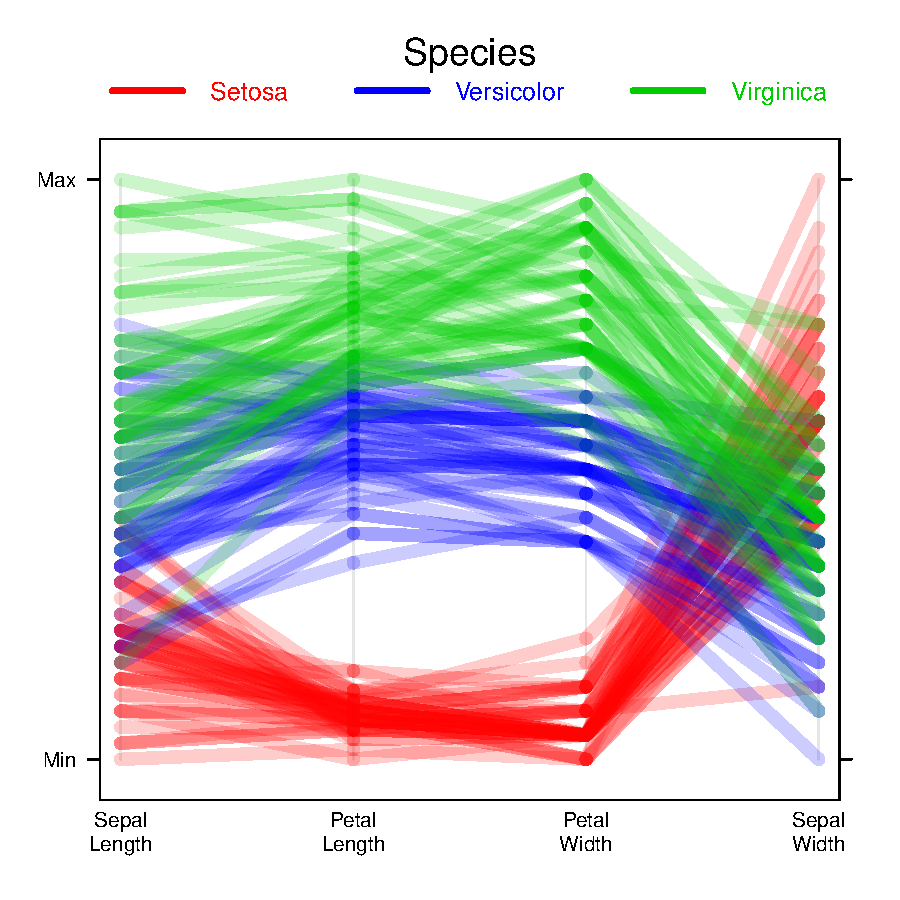
\includegraphics[width=.49\textwidth]{ch01/fig/iris-parallel-2} }

\caption[Parallel coordinates plots of the Iris data]{Parallel coordinates plots of the Iris data. Left: Default variable order; right: Variables ordered to make the pattern of correlations more coherent.\label{fig:iris-parallel}}
\end{figure}


\end{knitrout}
Parallel coordinate plots for categorical data are discussed in 
an online supplement on the web site for the book.
%\secref{sec:parallel}.
A general method for reordering variables in multivariate data visualizations based on
cluster analysis was proposed by \citet{Hurley:2004}.


\end{Example}

\subsection{Interactive and dynamic graphics}\label{sec:intro-interactive}

%\subsection{Interactive and dynamic graphics}\label{sec:intro-interactive}

Graphics displayed in print form, such as this book, are necessarily static
and fixed at the time they are designed and rendered as an image.
Yet, recent developments in software, web technology and media
alternative to print have created the possibility to extend graphics
in far more useful and interesting ways, for both presentation
and analysis purposes.

Interactive graphics\ix{interactive graphics}\ix{graphics!interactive}
allow the viewer to directly manipulate the
statistical and visual components of graphical display.  These
range from
\begin{itemize*}
\item graphical controls (sliders, selection boxes and other widgets)
to control details of an analysis (e.g., a smoothing parameter) or graph
(colors and other graphic details), to
\item higher-level interaction including zooming in or out,
drilling down to a data subset,
linking multiple displays, selecting terms in a model and so forth.
\end{itemize*}
The important effect is that the analysis and/or display is immediately
re-computed and updated visually.

In addition, \term{dynamic graphics} use animation to show a series of
views, as frames in a movie.  Adding time as an additional
dimension allows far more possibilities, for example
showing a rotating view of a 3D graph or showing smooth transitions
or interpolations from one view to another.

There are now many packages in \R providing interactive and dynamic plots
(e.g., \pkg{rggobi}, \pkg{iplots})
as well as capabilities to incorporate these into interactive documents,
presentations and web pages (e.g., \pkg{rCharts}, \pkg{googleVis}, \pkg{ggvis}).
The \Rpackage{animate} facilitates creating animated graphics  and movies in a
variety of formats.
The RStudio editor and development environment%
\footnote{\url{http://www.rstudio.com}}
provides its own
\Rpackage{manipulate}, as well as the \pkg{shiny} framework for
developing interactive \R web applications.

\begin{Example}[512paths]{512 paths to the White House}
Shortly before the 2012 U.S. presidential election (November 2, 2012)
the \emph{New York Times} published an interactive graphic%
\footnote{\url{http://www.nytimes.com/interactive/2012/11/02/us/politics/paths-to-the-white-house.html}},
designed by Mike Bostock and Shan Carter%
\footnote{
see: \url{https://source.opennews.org/en-US/articles/nyts-512-paths-white-house/}
for a description of their design process.}
showing
the effect that a win for Barack Obama or Mitt Romney in the
nine most highly contested states would have on the chances
that either candidate would win the presidency.

\begin{figure}
\centering
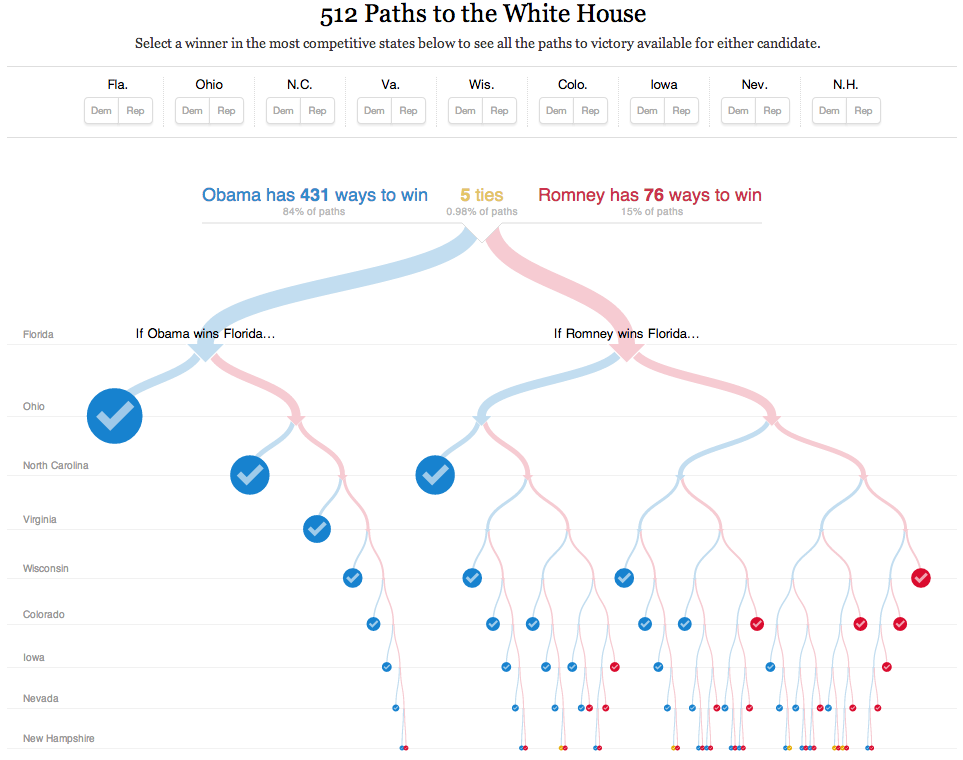
\includegraphics[width=0.7\textwidth]{ch01/fig/nyt_512paths.png}
\caption{512 paths to the White House.  This interactive graphic allows the viewer to
select a winner in any one or more of the nine most highly contested U.S. states
and highlights the number of paths leading to a win by Obama or Romney, sorted and
weighted
by the number of Electoral College votes.}
\label{fig:nyt_512paths}
\end{figure}

With these nine states in play there are $2^9 = 512$ possible outcomes,
each with a different number of votes in the Electorial College.
In \figref{fig:nyt_512paths}, a win for Obama in Florida and Virginia was
selected, with wins for Romney in Ohio and North Carolina.
Most other selections also lead to a win by Obama, but those with
the most votes are made most visible at the top.
An \R version of this chart was created using the \Rpackage{rCharts}.%
\footnote{
\url{http://timelyportfolio.github.io/rCharts_512paths/}
}
The design of this graphic as a \term{binary tree} was chosen here, but
another possibility would be a \term{treemap} graphic
\citep{Shneiderman:92} or a mosaic plot.


\end{Example}




\subsection{Visualization = Graphing + Fitting + Graphing $\dots$}\label{sec:vis}
\epigraph{Look here, upon this picture, and on this.}{Shakespeare, Hamlet}

Statistical summaries, hypothesis tests, and the numerical parameters
derived in fitted models are designed to capture a particular feature of the
data.  A quick analysis of the data from \tabref{tab:berk220}, for example,
shows that
1198/2691~=~44.5\% of male applicants were admitted, compared to
557/1835~=~30.4\% of female applicants.

Statistical tests
give a Pearson $\chi^2$ of 92.2
with 1 degree of freedom
for association between admission and gender ($p < 0.001$), and
various measures for the strength of association.
% <<UCBstats>>=
% UCB <- margin.table(UCBAdmissions, 1:2)
% assocstats(UCB)
% oddsratio(UCB, log=FALSE)
% @
%
Expressed in terms of the \term{odds ratio}, males were apparently
1.84 times as likely
to be admitted as females, with 99\% confidence bounds
$\left(1.56, 2.17\right)$.
Each of these numbers expresses some part of the relationship between
gender and admission in the Berkeley data.
Numerical summaries such as these are each
designed to compress the information in the data, focusing on some particular
feature.
%\TODO{Use this for a lab exercise in Ch 2.}

In contrast, the visualization approach to data analysis is designed
to
\begin{seriate}
\item expose information and structure in the data,
\item supplement the information available from numerical summaries, and
\item suggest more adequate models.
\end{seriate}
In general, the visualization approach seeks to serve the needs of
both summarization and exposure.

This approach recognizes that both data analysis and graphing are
\emph{iterative} processes.
You should not expect that any one model captures all features of the
data, any more than we should expect that a single graph shows all that
may be seen.  In most cases, your initial steps should include some
graphical display guided by understanding of the subject matter
of the data.
What you learn from a graph may then help suggest features of the data
to be incorporated into a fitted model.
Your desire to ensure that the fitted model is an adequate summary
may then lead to additional graphs.

The precept here is that
\precept{Visualization = Graphing + Fitting + Graphing $\dots$}
where the ellipsis indicates the often iterative nature of this process.
Even for descriptive purposes, an initial fit of salient features can be
removed from the data, giving residuals (departures from a model).
Displaying the residuals may then suggest additional features to account for.

Simple examples of this idea include detrending time series graphs to remove
overall and seasonal effects and plots of residuals from main-effect models
for ANOVA designs.  For categorical data, mosaic plots (\chref{ch:mosaic})
display the unaccounted-for association between variables by shading,
as in \figref{fig:glass-mosaic}.  Additional models and plots
considered in \secref{sec:loglin-square} can reveal additional structure
in square tables beyond the obvious effect that sons tend most often to
follow in their fathers' footsteps.

\begin{Example}[donner0a]{Donner Party}
The graphs in \figref{fig:donner0} and \figref{fig:donner0-other}
suggest three different initial descriptions for survival in the
Donner party.  Yet they ignore all other influences, of which
gender and family structure might also be important.
A more complete understanding of this data can be achieved
by taking these effects into account, both in fitted models
and graphs.  See \exref{ex:donner1} for a continuation of this story.
\end{Example}

\begin{Example}[nasa]{Space shuttle disaster}

The space shuttle \emph{Challenger} mentioned in \exref{ex:nasa0}
exploded 73 seconds after take-off on
January 28, 1986.
Subsequent investigation presented to the presidential commission
headed by William Rogers
determined that the cause was failure of the O-ring
seals used to isolate the fuel supply from burning gases.
The story behind the \emph{Challenger} disaster is perhaps the most poignant
missed opportunity in the history of statistical graphics.
See \citet{Tufte:97} for a complete exposition.
It may be heartbreaking to find out that some important information
was there, but the graph maker missed it.

\begin{figure}[htb]
  \centering
  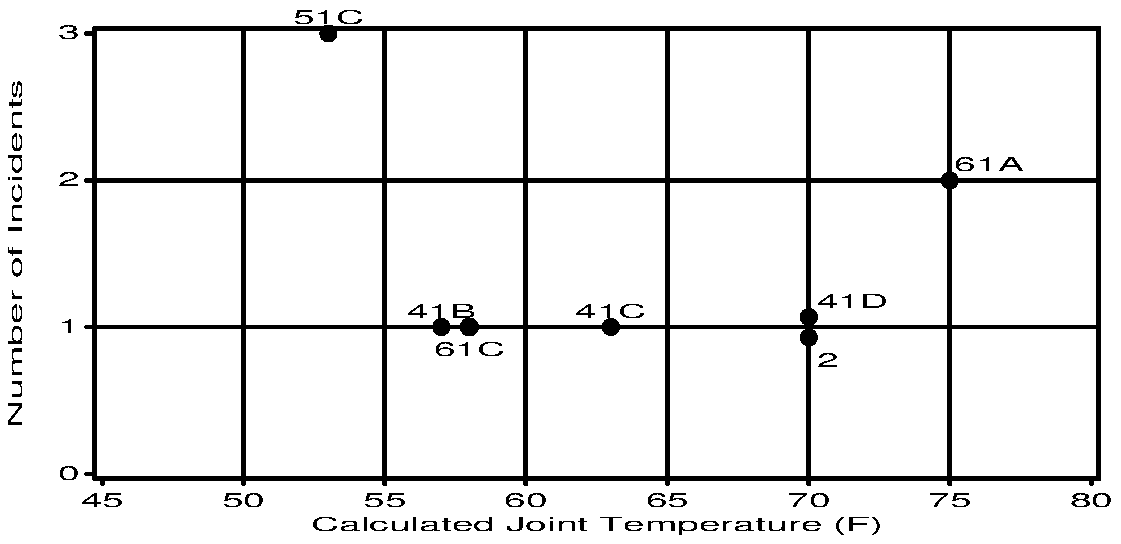
\includegraphics[width=\textwidth,clip]{ch01/fig/nasa0}
  \caption{NASA Space Shuttle pre-launch graph prepared by the engineers at Morton Thiokol.
%   \TODO{PC: the aspect ratio makes the graph really stretched (unless this is deliberate). It looks like the problem is in the nasa0 image itself; redownload/redraw? FIXME}
  }\label{fig:nasa0}
\end{figure}

Engineers from Morton Thiokol, manufacturers of the rocket motors,
had been worried about the effects of unseasonably cold weather
on the O-ring seals and recommended aborting the flight.
NASA staff analysed the data, tables and charts submitted by
the engineers and concluded that there was insufficient evidence
to cancel the flight.

The data relating O-ring failures to temperature were depicted as in
\figref{fig:nasa0}, our candidate for the most misleading graph in history.
There had been 23 previous launches of these rockets giving data on
the number of O-rings (out of 6) that were seen to have suffered
some damage or failure. However, the engineers omitted the observations
where no O-rings failed or showed signs of damage, believing that they were uninformative.

Examination of this graph seemed to indicate that there was no relation
between ambient temperature and failure.
Thus, the decision to launch
the \emph{Challenger} was made, in spite of the initial concerns
of the Morton Thiokol engineers.
Unfortunately, those observations had occurred when the launch temperature
was relatively warm (\degree{65-80}F.) and were indeed informative.
The coldest temperature at any previous launch was \degree{53};  when \emph{Challenger} was launched on January 28,
the temperature was a frigid \degree{31}.

These data have been analyzed extensively
\citep{Dalal-etal:89,Lavine:91}.
\citet{Tufte:97} gives a thorough and convincing
visual analysis of the evidence available prior to the launch.
We consider statistical analysis of these data in \chref{ch:logistic},
\exref{ex:nasa-temp}.

But, what if the engineers had simply made a better graph?
At the very least, that would entail
\begin{seriate}
\item drawing a smoothed curve to fit the points (to show the trend)
\item removing the background grid lines (which obscure the data).
\end{seriate}
\figref{fig:nasa}
shows a revised version of the same graph, highlighting
the non-zero observations and adding a simple quadratic
curve to allow for a possible non-linear relationship.
For comparison, the excluded zero observations are also
shown in grey.
This plot, even showing only the non-zero points
should have caused any engineer to conclude that
either:
\begin{seriate}
\item the data were wrong, or
\item there were excessive risks
associated with both high and low temperatures.
\end{seriate}
But it is well-known
that brittleness of the rubber used in the O-rings is inversely
proportional to Temperature cubed, so prudent interest might have focussed
on the first possibility.%
%\DONE{Add coda: Feynman O-ring demonstration to the Rogers Commission}
\footnote{A coda to this story shows the role of visual explanation in practice as well
\citep[p. 50--53]{Tufte:97}.
The Rogers Commission contracted the reknown theoretical physicist Richard Feynman
to contribute to their investigation.  He determined that the most probable
cause of the shuttle failure was the lack of resiliancy of the rubber O-rings
at low temperature. But how could he make this point convincingly?
At a televised public hearing, he took a piece of the O-ring material,
squeezed it in C-clamp and plunged it into a glass of ice water.
After a few minutes, he released the clamp, and the rubber did not spring
back to shape.  He mildly said,
``... there is no resilience in this particular material when it is at a
temperature of 32 degress. I believe this has some significance for our
problem'' \citep{Feynman:1988}.
}

\begin{figure}[htb]
  \centering
  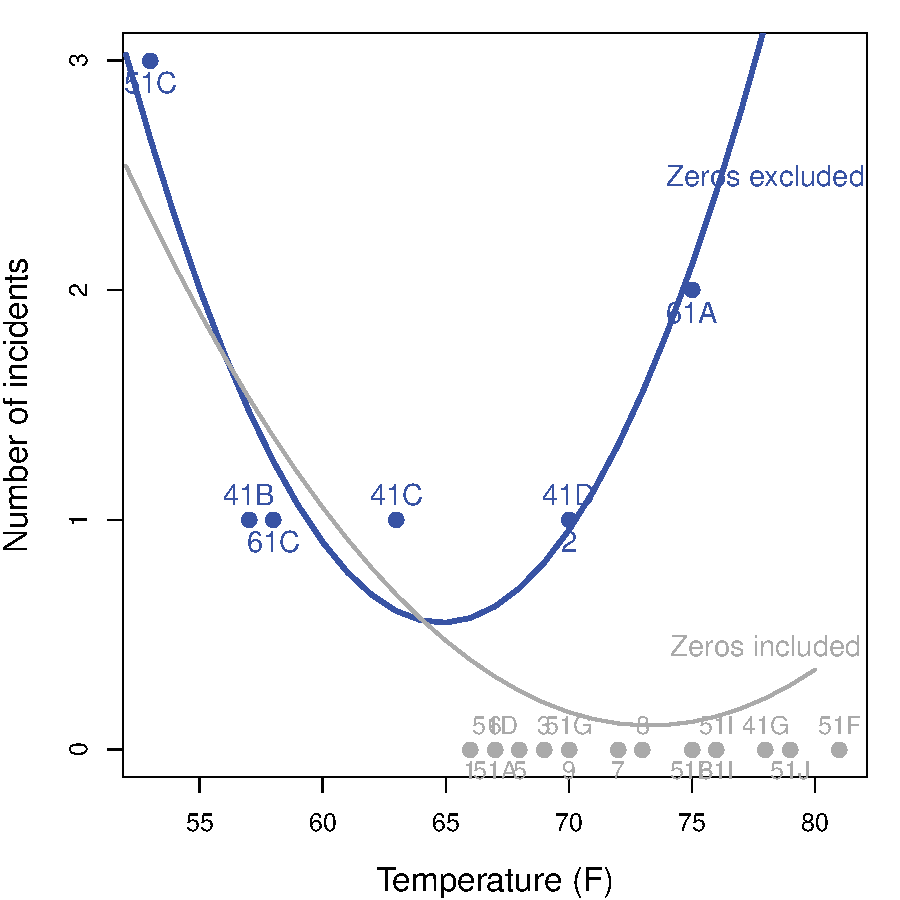
\includegraphics[width=.7\textwidth,clip]{ch01/fig/nasa}
  \caption{Re-drawn version of the NASA pre-launch graph, showing the locations of the excluded observations and with fitted quadratics for both sets of observations}\label{fig:nasa}
\end{figure}

%\DONE{DM: Maybe remove coda: example is quite long already. MF: Made a footnote}

\end{Example}

\subsection{The 80-20 rule}
The Italian economist Vilfredo Pareto observed in 1906 that 80\% of the land in Italy was
owned by 20\% of the population and this ratio also applied in other countries. 
It also applied to the yield of peas from peapods in his garden \citep{Pareto:1971}.
This idea became known as the
\term{Pareto principle} or the \term{80--20 rule}.
The particular 80/20 ratio is not as important as the more general idea of the
uneven distribution of results and causes in a variety of areas.

Common applications are the rules of thumb that: 
\begin{seriate}
  \item in business 80\% of sales come from 20\% of clients; 
  \item in criminology 80\% of crimes are said to be committed by 20\% of the population.
  \item In software development, it is said that 80\% of errors and 
  \item crashes can be eliminated by fixing the top 20\% most reported bugs
or that 80\% of errors reside in 20\% of the code.
\end{seriate}

The \term{Pareto chart} was designed to display the frequency distribution of
a variable with a histogram or bar chart together with a cumulative line graph
to highlight the most frequent category, and the \term{Pareto distribution}
gives a mathematical form to such distributions with a parameter $\alpha$
(the \emph{Pareto index})
reflecting the degree of inequality.

Applied to statistical graphics, the precept is that
\precept{20\% of your effort can generate
80\% of your desired result in producing a given plot.}
This is good news for exploratory
graphs you produce for yourself.  Very often, the default settings will give a reasonable
result, or you will see immediately something simple to add or change to make the plot
easier to understand.

The bad news is the corollary of this rule:
\precept{
80\% of your effort may be required to produce the remaining 20\% of a finished graph.
}
This is particularly important for presentation graphs, where several iterations
may be necessary to get it right (or right enough) for your communication purposes.
Some important details are:
\begin{description}

\item[graph title] A presentation graphic can be more effective when it announces
 the main point or conclusion in the graphic title, as in \figref{fig:arrests0-star}.

\item[axis and value labels] Axes should be labelled with meaningful variable descriptions
 (and perhaps the data units) rather than just plot defaults (e.g., ``Temperature (degrees F)''
 in \figref{fig:spaceshuttle0}, not \code{temp}).
 Axis values are often more of a challenge for categorical variables, where their text
 labels often overlap, requiring abbreviation, a smaller font or text rotation.

\item[grouping attributes] Meaningfully different subsets of the data should be
 rendered with distinct visual attributes such as color, shape, and line style,
 and sometimes with more than one.

 \item[legends and direct labels] Different data groups in a graphic display
 shown by color, shape, etc.  usually need at least a graphic legend defining
 the symbols and group labels. Sometimes you can do better by applying the
 labels directly to the graphical elements,%
 \footnote{
 For example, the \func{identify} function allows points in a plot to be labeled
 interactively with a mouse.  The \Rpackage{directlabels} provides a general
 method for a variety of plots.
 }
 as was done in \figref{fig:nasa}.

 \item[legibility] A common failure in presentation graphs in journals
 and lectures is the use of text fonts too small to be read easily.
 One rule of thumb is to hold the graph at arms length for a journal
 and put it on the floor for a lecture slide.  If you can't read the
 labels, the font is too small.

 \item [plot annotations] Beyond the basic graphic data display, additional
 annotations can add considerable information to interpret the context
 or uncertainty, as in the use of plot envelopes to show confidence bands
 or regions (see \figref{fig:donner0} and \figref{fig:donner0-other}).

 \item[aspect ratio] Line graphs (such as \figref{fig:arbuthnot1})
 are often easiest to understand when the ratio of
 height to width is such that line segments have an average slope
 near 1.0 \citep{Cleveland-etal:88:shape}.
 In \R, you can easily manipulate a graph window manually with a
 mouse to observe this effect and find an aspect ratio that looks
 right.

 Moreover, in graphs for biplots and \ca (\chref{ch:corresp}),
 interpretation involves distances between points and
 angles between line segments. This requires an aspect ratio
 that equates the units on the axes.  Careful software will
 do this for you,%
 \footnote{
 For example using the graphics parameter \code{asp=1},
 \func{eqsplot} in \pkg{MASS},
 or the equivalents in \pkg{lattice} (\code{aspect="iso"})
 and \pkg{ggplot2} (\code{coord\_equal}).
 }
 and you should resist the temptation to re-shape the plot.

\item[colors] Whereas a good choice of colors can greatly enhance a
  graphical display, badly-chosen colors, ignoring principles of 
  human perception, can actually spoil it. First, considering that
  a significant percentage of the human population
  is affected by color deficiencies, important information should
  never be coded by color alone. Second, color palettes should be
  chosen carefully to put the desired emphasis on the information 
  visualized. For example, consider \figref{fig:colors}
  showing qualitative color palettes 
  (appropriate for unordered categories)
  taken from two different color spaces: Hue-Saturation-Value (HSV) 
  and Hue-Chroma-Luminance (HCL), where only the hue is varied. 
  Whereas one would expect such a palette to be
  balanced with respect to colorfulness and
  brightness, the red colors in the left (HSV) 
  color wheel are generally perceived to
  be more more intense and flashy than the corresponding blue
  colors, and the highly saturated dark blue dominates the wheel.
  Consequently, areas shaded with these colors may appear more
  important than others in an uncontrolled way, distracting from the
  information to be conveyed. In contrast, the colors from the right (HCL)
  wheel are all balanced to the same gray level and in
  ``harmony''. These clearly should be preferred whenever categories of the
  same importance shall be compared.
  Another related perception rule prescribes that lighter and darker colors
  should not be mixed in a display
  where areas should be compared since lighter colors look larger than
  darker ones. More background information on the
  choice of ``good'' colors for statistical graphics 
  can be found in \citet{Zeileis-etal:2009}.
  
\item[visual impact] Somewhat related,
  important features of a display 
  should be distinguished from the less important. This may be
  achieved by different color or gray shading levels, 
  or simply by contrasting
  filled with non-filled geometric shapes, or a different density of
  shading lines. As a consequence, displays should never be overloaded
  with filled areas, so that the important ones can stand out.

\begin{knitrout}
\definecolor{shadecolor}{rgb}{1, 0.961, 0.933}\color{fgcolor}\begin{figure}[!htbp]

\centerline{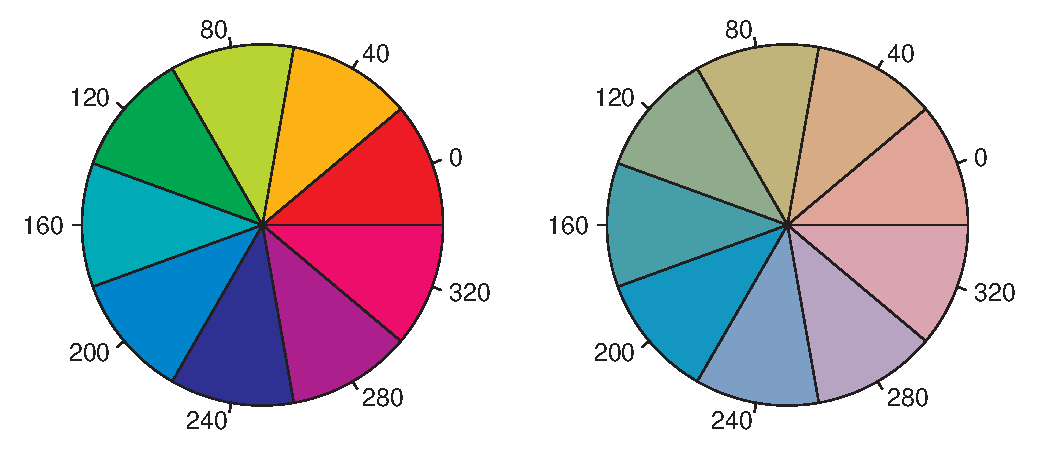
\includegraphics[width=.8\textwidth]{ch01/fig/colors-1} }

\caption[Qualitative color palette for the HSV (left) and HCL (right) spaces]{Qualitative color palette for the HSV (left) and HCL (right) spaces. The HSV colors are $(H, 100, 100)$ and the HCL colors $(H, 50, 70)$ for the same hues $H$. Note that in a monochrome version of this paper, all pies in the right wheel will be shaded with the same gray, i.e., they will appear to be virtually identical.\label{fig:colors}}
\end{figure}


\end{knitrout}
 
\end{description}

Nearly all of the graphs in this book were produced using \R code in
scripts saved as files.  This has the advantages of reproducibility
and enhancement: just re-run the code, or tweak it to improve a graph.
If this is too hard, you can always use an external graphics editor
(Gimp, Inkscape, Adobe Illustrator, etc.) to make improvements manually.

\section{Chapter summary}
%\Section{Chapter summary}

\begin{itemize}

  \item Categorical data differs from quantitative data because the variables take on
  discrete values (ordered or unordered, character or numeric)
  rather than continuous numerical values. Consequently,
  such data often appear in aggregated form representing category frequencies or in tables.

  \item Data analysis methods for categorical data are comprised of those concerned mainly
  with testing particular hypotheses versus those that fit statistical models.
  Model building methods have the advantages of providing parameter estimates and
  model-predicted values, along with measures of uncertainty (standard errors).

  \item Graphical methods can serve different purposes for different goals
  (data analysis versus presentation), and these suggest different design
  principles that a graphic should respect to achieve a given communication goal.

  \item For categorical data, some graphic forms (bar charts, line graphs,
  scatterplots) used for quantitative data can be readily adapted to
  discrete variables.
  However, frequency data often requires novel graphics using area and other
  visual attributes.

  \item Graphics can be far more effective when categorical variables are ordered
  to facilitate comparison of the effects to be seen and rendered to facilitate
  detection of patterns, trends or anomalies.

  \item The visualization approach to data analysis often entails a sequence of
  intertwined steps  involving graphing and model fitting.

  \item Producing effective graphs for presentation is often hard work, requiring
  attention to details that support or detract from your communication goal.
\end{itemize}


\section{Further reading}\label{sec:ch01-reading}


\section{Lab exercises}\label{sec:ch01-exercises}
% These exercises have no code
%\section{Lab exercises}\label{sec:ch01-exercises}

\begin{Exercises}

 \exercise A web page, ``The top ten worst graphs, '' \url{http://www.biostat.wisc.edu/~kbroman/topten_worstgraphs/} by Karl Broman lists his picks for the worst graphs (and a table) that have appeared in the
 statistical and scientific literature.  Each entry links to graph(s) and a brief discussion of
 what is wrong and how it could be improved. 
 \begin{enumerate*}
   \item Examine a number of recent issues of a scientific or statistical journal in which you
   have some interest.  Find one or more examples of a graph or table that is a particularly
   bad use of display material to summarize and communicate research findings. Write a
   few sentences indicating how or why the display fails and how it could be improved.
   \item Do the same task for some popular magazine or newspaper that uses data displays
   to supplement the text for some story. Again, write a few sentences describing why the
   display is bad and how it could be improved.
 \end{enumerate*}
 
 \exercise As in the previous exercise, examine the recent literature in recent issues of some
 journal of interest to you.  Find one or more examples of a graph or table that you feel
 does a \emph{good} of summarizing and communicating research findings.
 \begin{enumerate*}
   \item Write a few sentences describing why you chose these displays.
   \item Now take the role of a tough journal reviewer.  Are there any features of the
   display that could be modified to make them more effective?
 \end{enumerate*}
 
 \exercise Infographics are another form of visual displays, quite different from the
 data graphics featured in this book, but often based on some data or analysis.
 Do a Google image search for the topic ``Global warming'' to see a rich
 collection.
 \begin{enumerate*}
   \item Find and study one or two that attempt some visual explanation of causes
   and/or effects of global warming.  Describe the main message in a sentence or
   two.
   \item What visual and graphic features are used in these to convey the message?
 \end{enumerate*}

 \exercise The Wikipedia web page \url{en.wikipedia.org/wiki/Portal:Global_warming}
   gives a few data-based graphics on the topic of global warming.  
   Read the text and study the graphs.  
   \begin{enumerate*}
	   \item Write a short figure title for each that would announce the conclusion
	   to be drawn in a presentation graphic.  
	   \item Write a figure caption for each that 
	   would explain what is shown and the important graphical details for a reader to
	   understand.
   \end{enumerate*}

\end{Exercises}


%\TODO{Cleanup local variables}



















%%%%%%%%%%%%%%%%%%%%%%%%%%%%%%%%%%%%%%%%%%%%%%%%%%%%%%%%%%%%%%%%%%%%%%%%%


% To resolve citations in the chapter, ...
{\itemsep -1pt
\bibliography{graphics,statistics,timeref,Rpackages}
%%% Use aux2bib to process the .aux file, creating references.bib
%%% Then change to line below
%\bibliography{references}
}

% \newpage
% This document was produced using:
% 
% <<session-info>>=
% print(sessionInfo(), locale = FALSE)
% @

	
%%%%% THE END %%%%%
\end{document}

